\section{Umsetzung}
Das Architekturbild~\ref{fig:umsetzung_frontendarchitektur_4} auf Seite~\pageref{fig:umsetzung_frontendarchitektur_4}
zeigt die Architektur des Frontends und die Kommunikation mit dem API Connect Service. Dabei sollen sowohl das Frontend
als auch die Smartphone-Apps mit dem API-Gateway kommunizieren, um anfallende Anfragen zu vereinheitlichen.

Ein Cloud Foundry Container wird mit einem Node.js-Boilerplate versehen. Mit Hilfe des Boilerplates lassen sich
Node.js-Applikationen innerhalb des Containerts verwalten und nutzen. Es stellt eine Runtime zur Verfügung, in welcher
das Frontend laufen kann.

Die Smartphone-Apps werden auf Basis von Android und auch iOS entwickelt. Beide Systeme erhalten innerhalb der App ein
WebView-Layout, welche für das Laden und das Darstellen der Webseite zuständig ist. Damit ist es einfach, eine schon
erstellte, responsive Webseite optimal für ein Smartphone zu nutzen. Zusätzlich können Feinheiten wie angepasste Layouts
der einzelnen Systeme übernommen werden.

Die Kommunikation zwischen Frontend und API Connect sowie zwischen den entwickelten Smartphone-Apps und dem API Connect
Service laufen über REST-Aufrufe (englisch REST-Calls).

Da in den Smartphone-Apps lediglich das schon entwickelte Frontend geladen wird, müssen die Aufrufe nur ein Mal
spezifiziert und umgesetzt werden.

\begin{figure}[h]
    \centering
    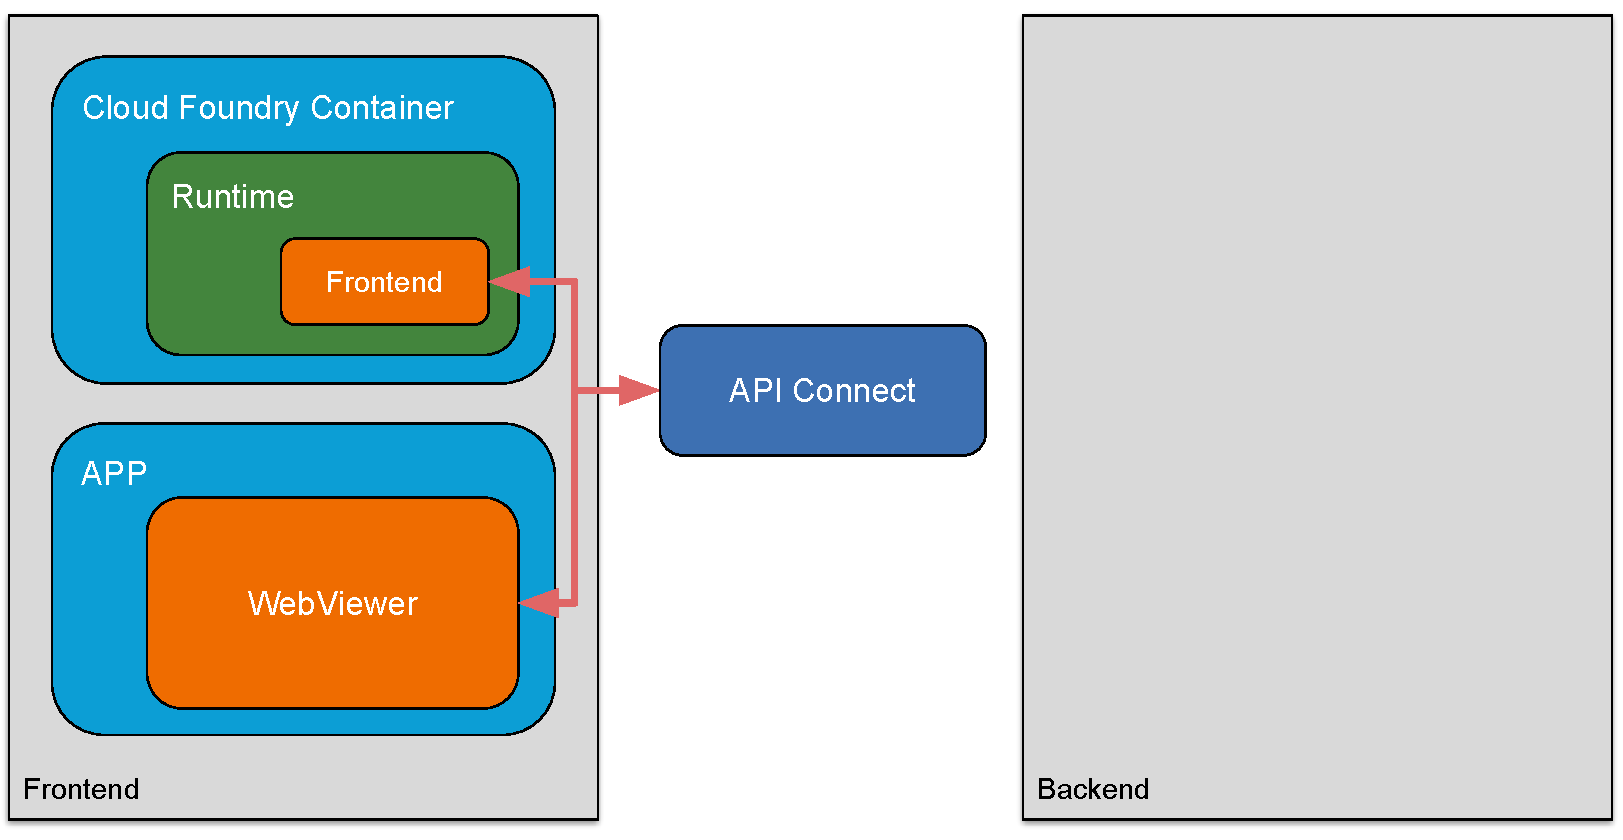
\includegraphics[width=\textwidth]{images/kapitel_4/architektur_frontend.pdf}
    \caption{Übersicht der Zielarchitektur}
    \label{fig:umsetzung_frontendarchitektur_4}
\end{figure}

\subsection{Web-Frontend}
\label{subsec:webseite}
Als nächstes kann man das Web-Frontend (auch Webseite oder englisch website oder auch client genannt) entwickeln. Um
nicht mit zahlreichen Iterationen und Anpassungen bei der Entwicklung zu kämpfen, empfiehlt es sich mit der Definition
von möglichen Use-Cases -- also mit der Definition von Aktionen eines Endnutzers auf der Webseite -- zu beginnen.

Anschließend sollte man für die einzelnen Use-Cases jeweils eigene Mockups erstellen die aufzeigen, wie ein Endnutzer
die einzelnen Aktionen durchführen kann. In einem weiteren Schritt setzt der Entwickler die gebauten Mockups dann in
Quellcode um, damit ein Prototyp entsteht. Diesen könnte man dann mit einer ausgewählten Gruppe testen, um wertvolles
Feedback zu erhalten.

Ein Test mit ausgewählten Nutzergruppen könnte Aufschluss darüber geben, wie gut der Prototyp bei einem Endnutzer
ankommt oder wie gut er Nutzbar ist. Dabei sollten man unter anderem auch Maschineneinsteller als Testpersonen
einsetzen, da diese die Zielgruppe für die Anwendung ist.

Damit die Benutzung der Webseite von verschiedenen Endgeräten aus optimal möglich ist, muss man sich im Weiteren
gedanken über das Thema \textit{Responsive} machen. Wie sich die gebaute Webseite also auf den verschiedenen
Displaygrößen selbstständig anpasst.

Nachdem man die Webseite dann fertig entwickelt hat, muss man sie noch in einen Container installieren. Dies ist über
mehrere Varianten möglich. Auch kann man zusätzliche Erweiterungen einbauen, welche das Arbeiten mit der Webseite
erleichtern oder speziellen Bedürfnissen der Endanwender gerecht wird.

\subsubsection{Use-Cases}
Als Use-Case kommt zum jetzigen Zeitpunkt lediglich eine Aktion in Frage. Das Erstellen von Vorhersagen für die manuell
eingetragenen Parameter der Maschine.

Da das Backend mit seinem neuronalen Netz und dem trainierten Modell aktuell nicht mehr berechnen kann, ist der
angegebene Use-Case auch der einzig sinnvolle.

Nachdem der Endnutzer die Parameter dann in ein Formular eingetragen hat, soll er die Möglichkeit bekommen, die
resultierenden Vorhersagen zu erhalten, um diese an der Maschine zu testen. Eine Fortschrittsanzeige soll darüber
informieren, dass das System arbeitet und der Anwender sich gedulden soll.

Da der Use-Case relativ einfach und schnell definiert werden konnte, kann man als nächstes mit der Erstellung der
Mockups für diesen beginnen. Es soll eine erste Idee und eine erste Umsetzung für die Anwendung basierend auf dem
Use-Case geben.

\subsubsection{Mockups erstellen}
Da der Use-Case nun definiert ist, kann man mit der Entwicklung des Mockups beginnen. Dabei ist die Wahl des
Designs auf eine zweispaltige Startseite gefallen. Eine der beiden Spalten beinhaltet die Eingabewerte und die andere
Spalte beinhaltet die vorhergesagten Argumente, welche das trainierte Modell bestimmt.

In Abbildung~\ref{fig:umsetzung_mockup_scale_1} auf Seite~\pageref{fig:umsetzung_mockup_scale_1} ist eine erste Version
des Frontends mit der Umsetzung der beiden Spalten zu sehen. Dabei werden in der linken Spalte die Werte in
Formularfelder eingetragen und in der rechten Spalte die vorhergesagten Parameter angezeigt.

Im mittleren Bereich der Seite soll ein Button erscheinen, welcher durch betätigen die eingetragenen Parameter an das
Backend schickt und anschließend den Output anzeigt.

\begin{figure}[h]
    \centering
    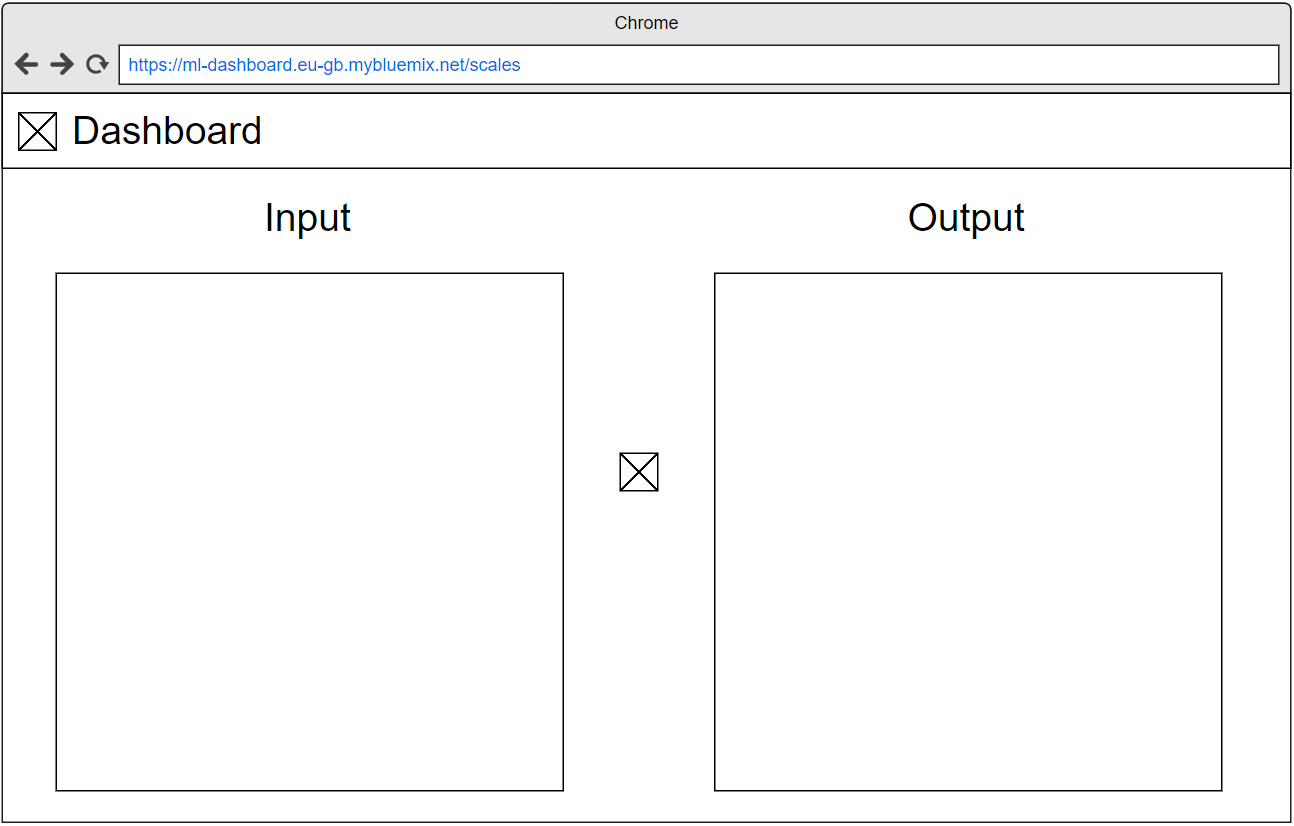
\includegraphics[width=\textwidth]{images/kapitel_4/mockup_scale_1.png}
    \caption{Erstes Mockup für das Dashboard}
    \label{fig:umsetzung_mockup_scale_1}
\end{figure}

Damit man sowohl den Input als auch den Output verbessert anzeigen kann ist es sinnvoll, die beiden Spalten noch weiter
zu unterteilen. Gerade bei den Eingabewerten gibt es zahlreiche Parameter, die man in Gruppen zusammenfassen kann.

So ist es zum Beispiel möglich die Parameter \textit{Produktbreite}, \textit{Produkthöhe} und \textit{Produkttiefe} zu
einer Gruppe namens \textit{Produktmaße} zusammen zu fassen.

Die Abbildung~\ref{fig:umsetzung_mockup_scale_2} auf Seite~\pageref{fig:umsetzung_mockup_scale_2} zeigt das angepasste
Mockup mit seinen Gruppen sowohl auf der Input"~ als auch der Output-Seite.

\begin{figure}[h]
    \centering
    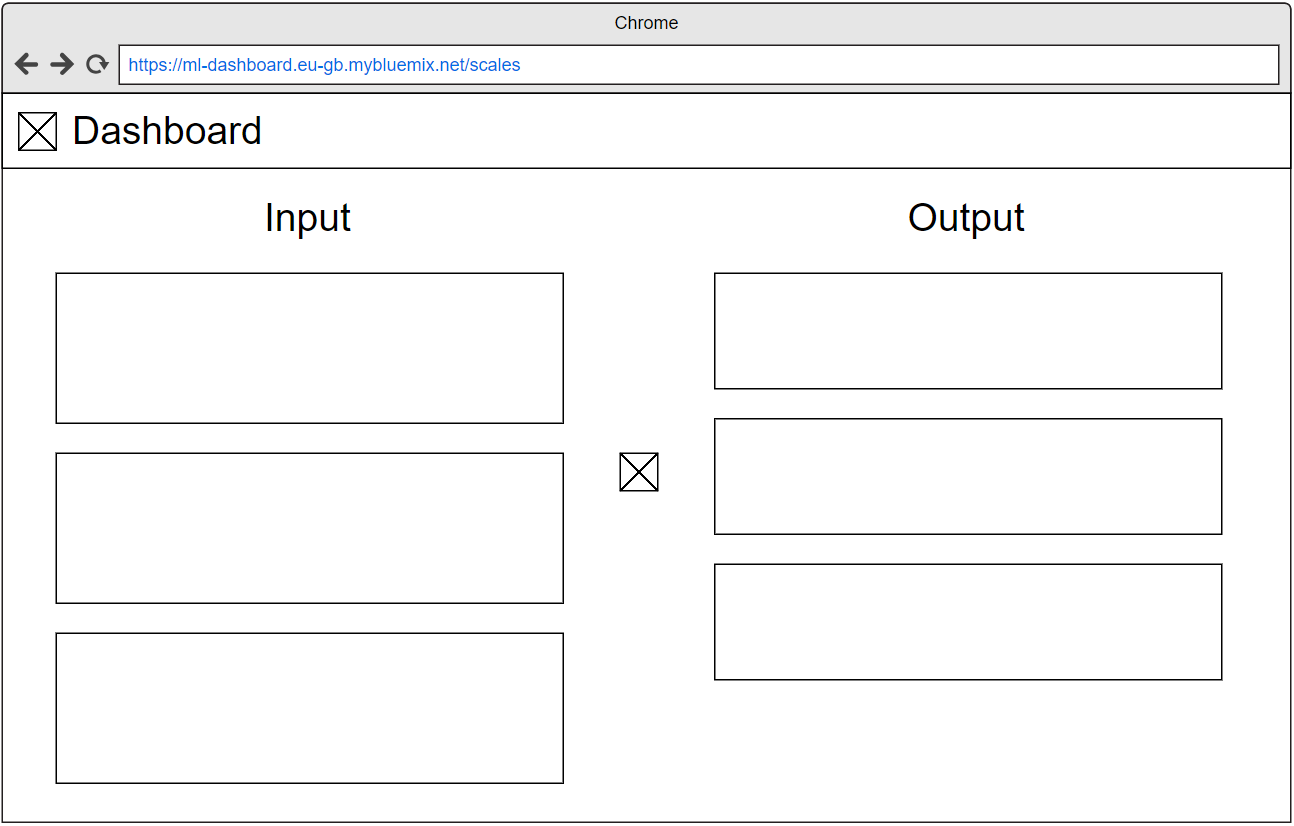
\includegraphics[width=\textwidth]{images/kapitel_4/mockup_scale_2.png}
    \caption{Überarbeitetes Mockup für das Dashboard}
    \label{fig:umsetzung_mockup_scale_2}
\end{figure}

Im oberen Bereich der Seite kann man ein Logo der Anwendung einbauen und nebenan den Namen für die aktuell geöffnete
Unterseite. So weiß der Anwender immer, auf welcher Seite er sich aktuell befindet.

Damit man das Frontend auch für weitere Maschinen oder Maschinenkomponenten erweitern kann, sollte der Entwickler ein
Menü hinzufügen, über das man auf die anderen Seiten mit Eingabe"~ und Ausgabewerte zugreifen kann.

Dieses Menü entwickelt man am Besten so, dass es sich aus dem linken Bereich herausschiebt und über ein
\textit{Hamburger-Menü-Icon}\footnote{https://de.wikipedia.org/wiki/Hamburger-Menü-Icon} zu öffnen ist. Dieses Symbol
hat mittlerweile Kultstatus erreicht und die meisten Anwender wissen damit umzugehen oder wissen was sie bei einem Klick
auf das Icon erwartet.

So ist in Abbildung~\ref{fig:umsetzung_mockup_scale_menu} auf Seite~\pageref{fig:umsetzung_mockup_scale_menu} das Mockup
für ein seitliches Menü zusammen mit dem darunterliegenden Inhalt zu sehen, welches über drei beispielhafte Menüeinträge
verfügt.

Das Menü soll sich beim Aufklappen über den Inhalt legen und den restlichen Bildschirm etwas ausgrauen sodass für den
Nutzer ersichtlich ist, dass er am Menü eine Auswahl treffen muss.

Ein Klick in den ausgegrauten Bereich, oder auch auf einen der Menüpunkte, schließt das Menü allerdings wieder, sodass
der Nutzer immer das tun kann, was er gerade möchte.

Die Auswahl eines neuen Menüpunktes hat außerdem zur Folge, dass sich die vorher angesprochene Überschrift im oberen
Bereich der Webseite mit dem Namen des Menüpunktes füllt, damit der Nutzer immer genau weiß, unter welchem Menüpunkt
er sich gerade befindet.

\begin{figure}[h]
    \centering
    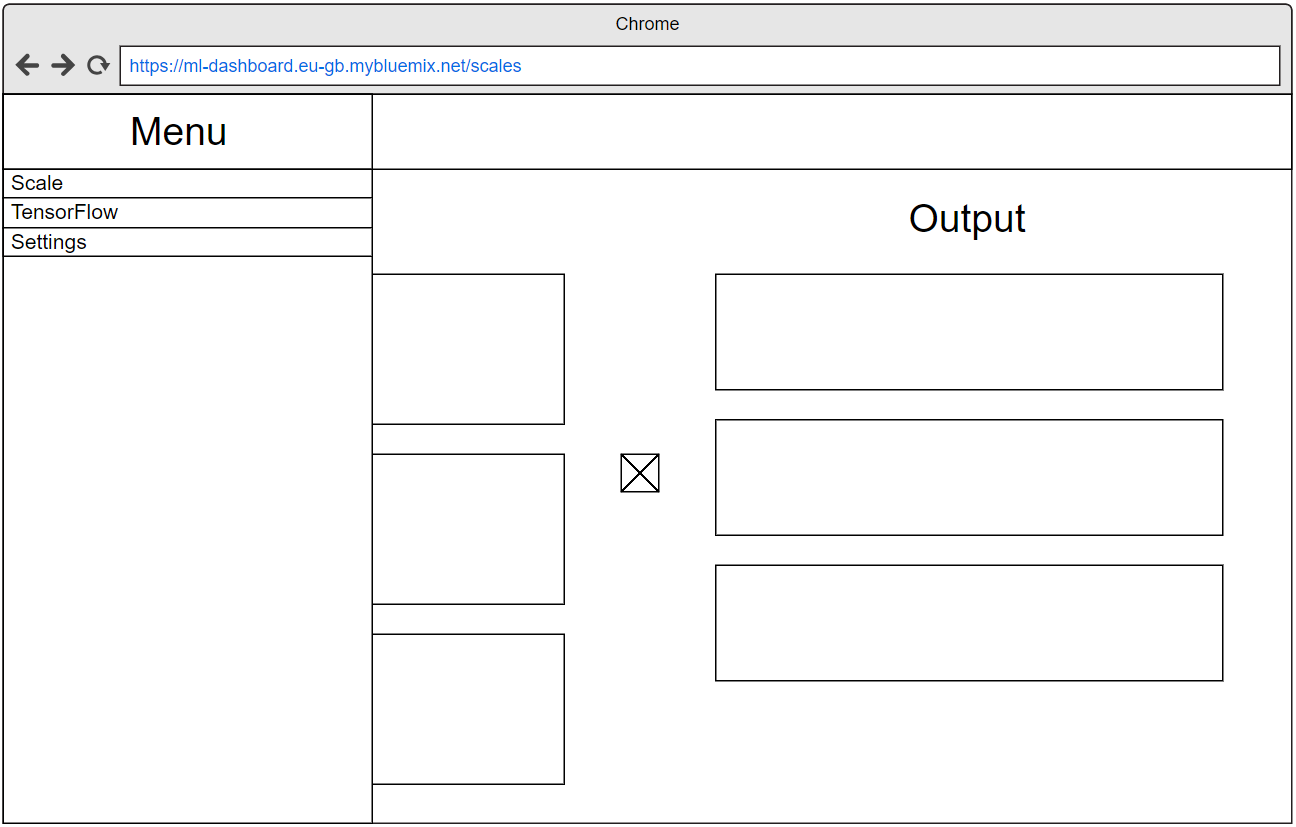
\includegraphics[width=\textwidth]{images/kapitel_4/mockup_scale_menu.png}
    \caption{Mockup für die Navigation}
    \label{fig:umsetzung_mockup_scale_menu}
\end{figure}

\subsubsection{Gedanken zu Responsive}
Damit das Frontend auch von einem Smartphone aus gut bedient und eine WebView-App dafür geschrieben werden kann, muss
die Webseite auf verschiedene Displaygrößen so reagieren können, damit es alle Informationen nutzerfreundlich und
akkurat anzeigt.

Dabei dürfen keine wichtigen Informationen verschwinden oder die Interaktion mit dem System eingeschränkt sein. Auch
sollte die Webseite sich optisch nicht zu sehr verändern als das der Nutzer der Meinung ist, dass er sich auf einer
andere Seite befindet.

Damit man dieser Anforderung gerecht werden kann, muss man das Frontend mit responsiven Eigenschaften versehen. Da die
Webseite in Ihrer ursprünglichen Idee zwei Spalten hat, ist es für die responsive Version interessant, die Spalten nicht
nebeneinander anzuzeigen, sondern untereinander.

Dies soll aber auch nur dann geschehen, wenn es nicht genügend Platz gibt, um beide Spalten nebeneinander anzuzeigen.

Bei größeren Displays wäre es im horizontalen Modus (englisch landscape mode) möglich, beide Spalten auch nebeneinander
darzustellen. Wohingegen im vertikalen Modus (englisch portrait mode) es immer Sinnvoll ist, die beiden Spalten
untereinander anzuzeigen.

Das Mockup in Abbildung~\ref{fig:umsetzung_mockup_scale_responsive} auf
Seite~\pageref{fig:umsetzung_mockup_scale_responsive} zeigt die Darstellung des Frontends auf einem Smartphone im
vertikalen Modus. Dabei ist die Spalte mit der \textit{Eingabe} aktuell sichtbar und unterhalb wird der Button für die
Berechnung der Ausgabeparameter angezeigt.

\begin{figure}[h]
    \centering
    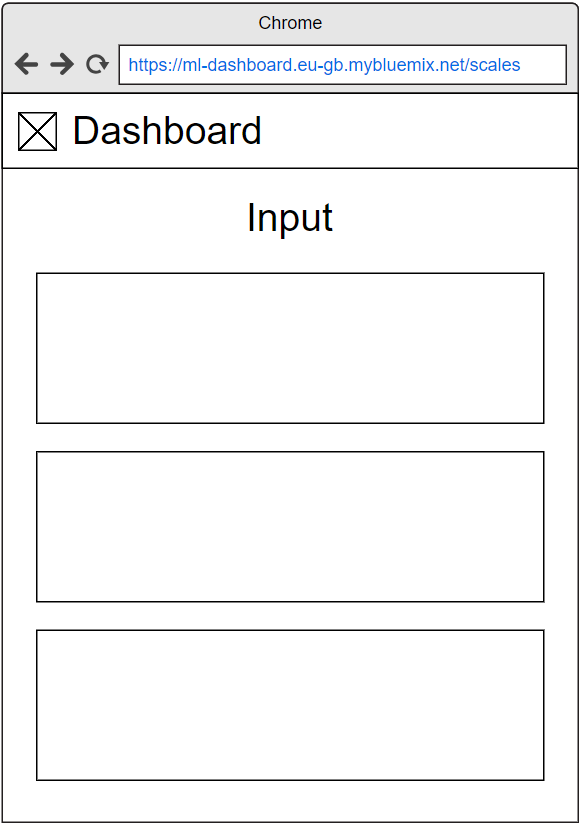
\includegraphics[scale=0.45]{images/kapitel_4/mockup_scale_responsive.png}
    \caption{Mockup des responsiven Designs}
    \label{fig:umsetzung_mockup_scale_responsive}
\end{figure}

Unter dem Button für das Absenden der Parameter ist die Spalte für die Ausgabeparameter angesiedelt welche erst
erscheint, wenn Vorhersagen aus dem Backend zur Verfügung stehen.

So ist der Scrollbalken auf der Webseite nicht unnötig lang und sorgt beim Endnutzer nicht für zusätzliche Verwirrung.
Auch wird so kein großer leerer Bereich auf der Webseite angezeigt, mit dem der Nutzer nichts anfangen kann.

Auch wird nach der Bestätigung des Buttons automatisch zum Bereich der Ausgabe gescrollt, damit dies nicht manuell
geschehen muss. Dabei handelt es sich um eine Komfortfunktion die man allerdings sehr einfach mit JavaScript umsetzen
kann.

\subsubsection{Webseite umsetzen}
Da die Mockups für die Anwendung fertig umgesetzt sind, kann im Weitern damit begonnen werden, das Frontend final
umzusetzen. Da man das Frontend mit Angular umsetzt und die Angular-CLI installiert ist, kann man auf dem
Entwicklerrechner mit dem folgenden Befehl eine neues Angular-Projekt einrichten.

\begin{lstlisting}[caption=Einrichten eines neuen Angular-Projektes, label=ls:umsetzung_angular]
    ng new dashboard
\end{lstlisting}

Dabei wird ein neuer Ordner mit dem Namen \textit{dashboard} angelegt, welcher alle benötigten Ordner und Dateien, um
eine funktionierende Angular-Seite zu bauen, beinhaltet.

Wenn man anschließend in den neu erstellen Ordner wechselt, kann man mit dem folgenden Befehl die Standard-Applikation
von Angular bauen lassen und sie im Browser ansehen.

\begin{lstlisting}[caption=Bereitstellen der Angular-Webseite, label=ls:umsetzung_angularserve]
    ng serve --open
\end{lstlisting}

Durch den Parameter \texttt{open} öffnet sich der Browser selbstständig und zeigt die Standardanwendung an. Darin ist
ein großes Bild des Angular-Logos mit einer großen Überschrift und ein paar weiteren Kommentaren zu sehen.

Jegliche Änderung am Quellcode der aktuellen Anwendung hat zur Folge, dass die entsprechende Angular-Komponente neu
gebaut und der Browser neu geladen wird um die Änderung direkt sichtbar zu machen.

Nun kann man damit beginnen, die Webseite entsprechend der Mockups umzusetzen. Dabei ist darauf zu achten, die
Standard-Komponenten der Angular-Material-Bibliothek zu nutzen. Somit ist sichergestellt, dass das Erscheinungsbild der
Anwendung einer Android-App ähnelt.

Die Komponenten sind auf der entsprechenden
Dokumentationsseite\footnote{https://material.angular.io/components/categories} zu finden und man kann sie von da aus
direkt kopieren um sie im eigenen Quellcode zu nutzen. Auch Icons und vorgefertigte Farben lassen sich der Webseite
entnehmen. Somit kann man sehr gut eine Android-App ähnliche Webseite aufbauen.

In Abbildung~\ref{fig:umsetzung_website_input} auf Seite~\pageref{fig:umsetzung_website_input} ist die fertig
umgesetzte Webseite zu sehen, in welcher ein Nutzer die Parameter für das neuronale Netz eingeben kann. Die linke Spalte
mit der \textit{Eingabe} ist also umgesetzt.

\begin{figure}[h]
    \centering
    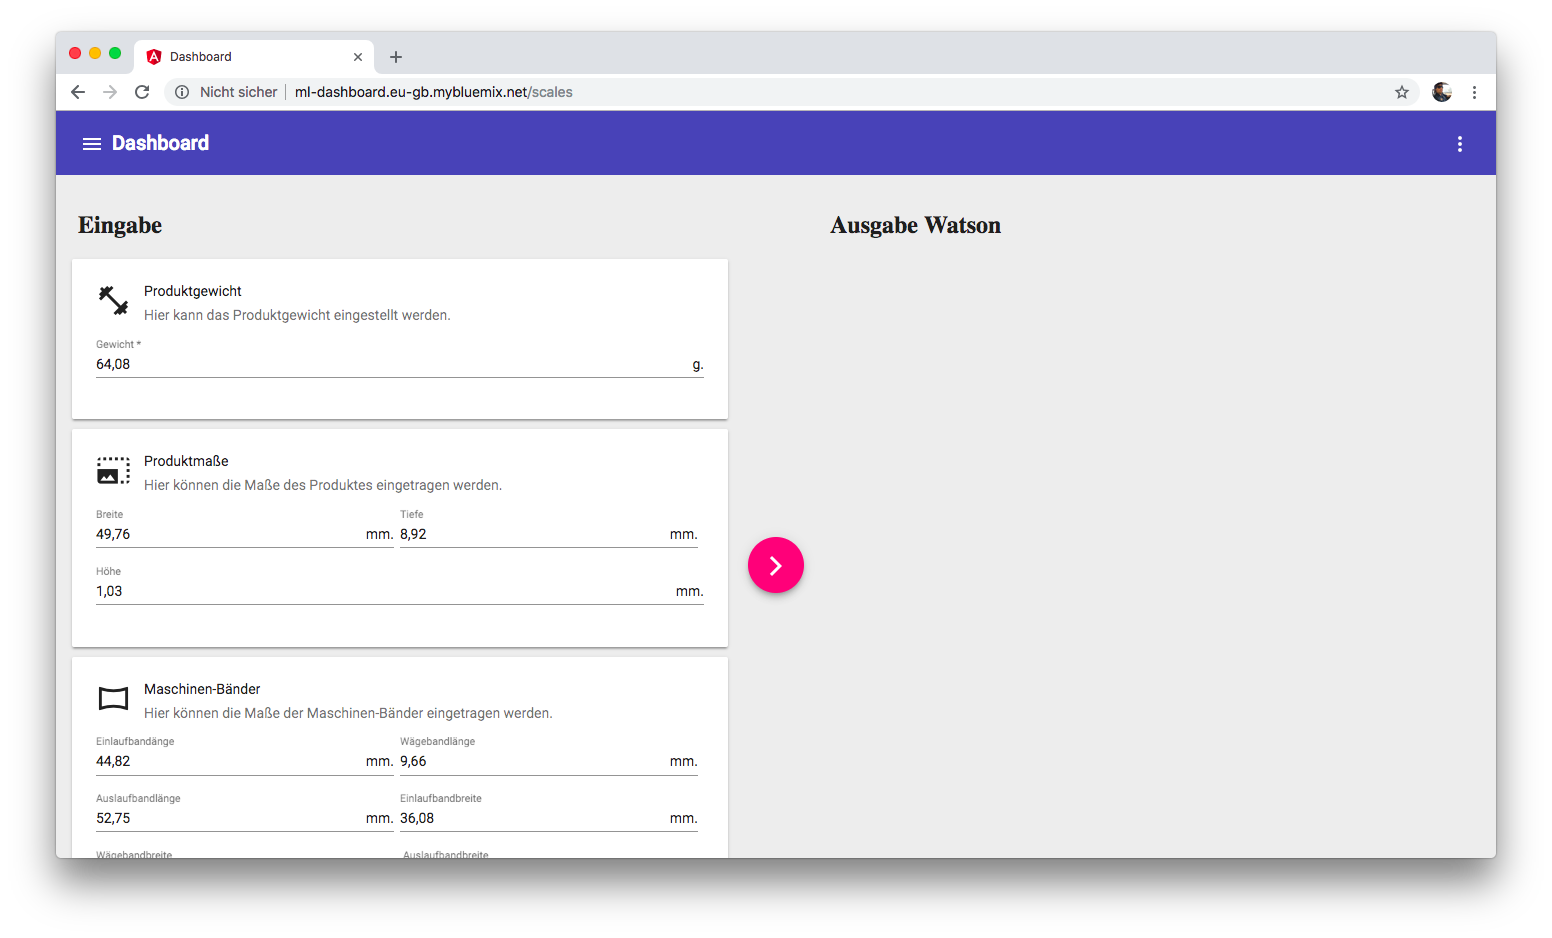
\includegraphics[width=\textwidth]{images/kapitel_4/website_input.png}
    \caption{Umsetzung der Webseite mit der Eingabe-Spalte}
    \label{fig:umsetzung_website_input}
\end{figure}

Nun kann man die zweite Spalte mit der \textit{Ausgabe} anfertigen um sie in dem noch leeren Platz zu positionieren. Die
Umsetzung ist dabei gleich der Umsetzung der linken Spalte in der Anwendung.

In der Abbildung~\ref{fig:umsetzung_website_output} auf Seite~\pageref{fig:umsetzung_website_output} ist die komplette
Webseite zu sehen mit beiden Spalten und dem Button zur generierung der Vorhersage.

\begin{figure}[h]
    \centering
    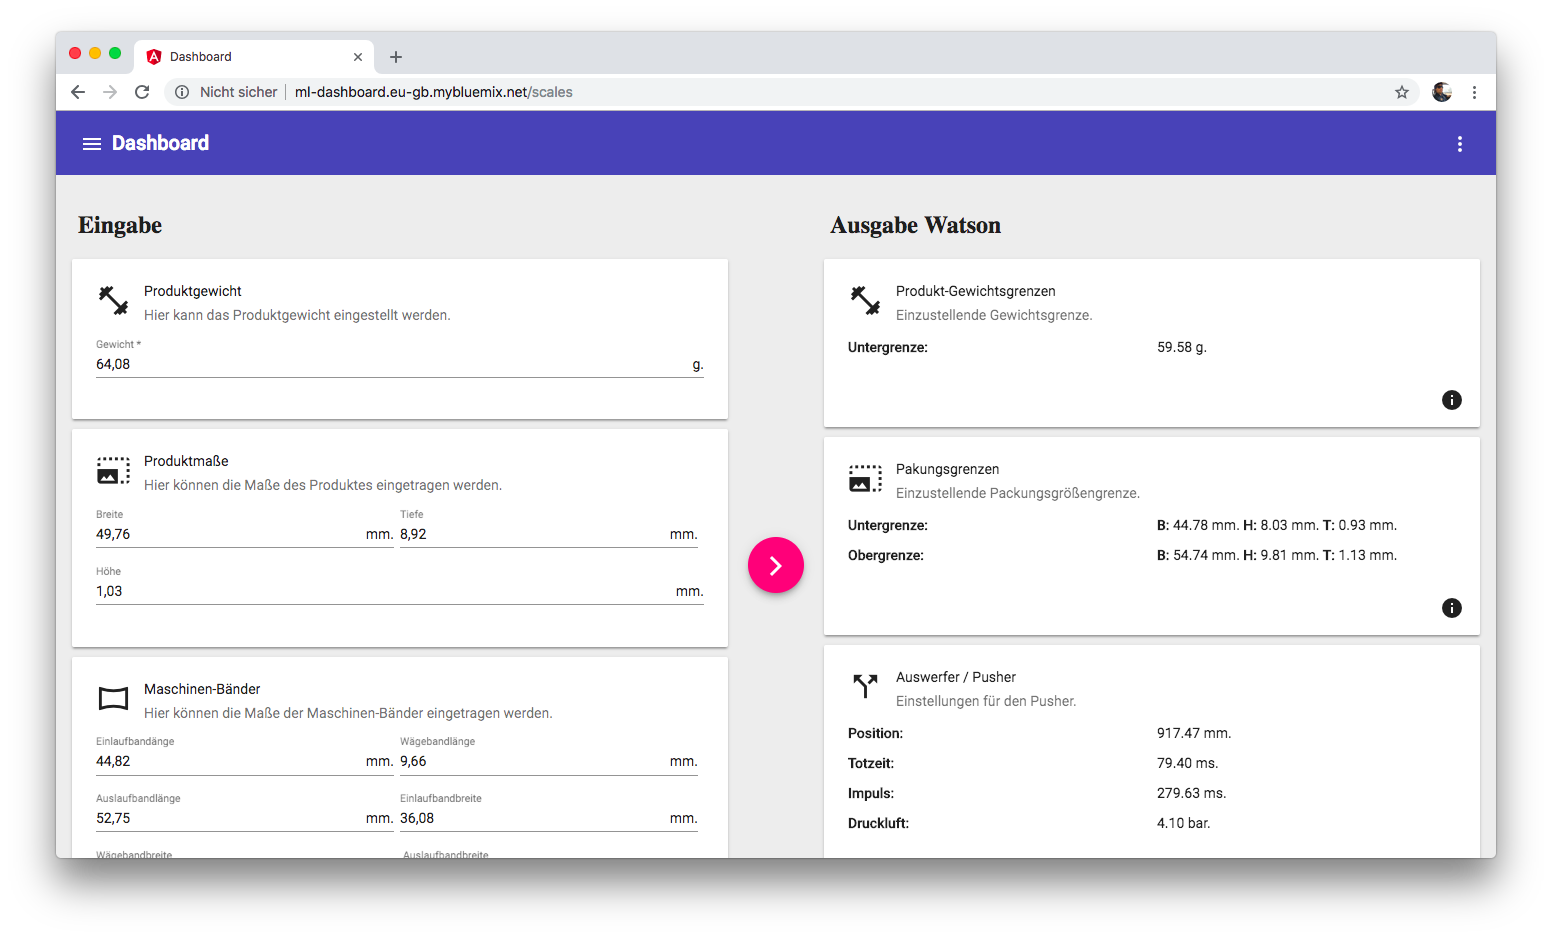
\includegraphics[width=\textwidth]{images/kapitel_4/website_output.png}
    \caption{Umsetzung der Webseite mit der Ausgabe-Spalte}
    \label{fig:umsetzung_website_output}
\end{figure}

Bei der Umsetzung ist entscheidend, dass die rechte Spalte des Dashboards nur dann angezeigt wird, wenn auch die Abfrage
an das Backend durch ist und Vorhersagen an das Frontend zurück gekommen sind.

Allerdings sollte man die Überschrift der Spalte -- Ausgabe -- anzeigen, damit der Endnutzer weiß dass da noch weitere
Informationen folgen werden.

Auch ist so für den Nutzer ersichtlich, dass der Platz auf der rechten Seite nicht verschwendet ist. Wenn sich die
Eingabe der Parameter über die gesamte Seite ziehen würde und sich dann nach betätigung des Buttons verkleinert, würde
das für zu viel bewegung in der Webseite führen.

Dies würde sich negativ auf das Verständnis der Webseite auswirken und zu manch komischen Darstellungen auf der Webseite
führen.

Die einzelnen Blöcke in der Spalte der Ausgabe erscheinen nach und nach durch kleine Animationen, welche die einzelnen
Boxen langsam einblendet. Dadurch kann man Zeit gewinnen, um das große JSON-Objekt, welches vom Backend zurück kommt,
komplett zu parsen.

Die einzelnen Werte muss man sich aus dem großen Array herausziehen um es an der passenden Stelle in der richtigen
Gruppe anzuzeigen.

Das Parsen kann zeitgleich mit der Animation starten. So wird dem Endnutzer symbolisiert, dass die Daten schon da sind
und sie auch gleich sichtbar sind. So muss er nicht noch das Parsing abwarten. Dies erleichtert die Arbeit mit der
Webseite auch dadurch enorm, als das Endnutzer nicht direkt mit vielen Boxen konfrontiert wird.

Desweiteren ist wichtig zu wissen, dass beim Aufruf der Seite in der Spalte für die Ausgabe noch keine Daten
bereitstehen. Darum macht die Darstellung des Bereichs auch keinen Sinn.

Damit der Endnutzer sich schneller auf der Webseite zurecht finden kann, ist die Platzierung von kleinen Icons und
Beschreibungstexten an den verschiedenen Boxen sinnvoll. So weiß der Nutzer direkt, was er in welcher Box machen oder
auch Einstellen kann.

Sinnvoll ist es auch die Parameter der linken Spalte mit passenden Zufallszahlen zu versehen. So kann der Nutzer direkt
nach dem öffnen der Seite eine Vorhersage starten um die Funktionsfähigkeit der Webseite und des Backends zu testen.

Auch kann er so nachvollziehen, welche Werte er in der linken Spalte eintragen muss, falls er sich zuanfang noch
unsicher über beispielsweise die Zahlengröße ist.

Als nächsten Schritt muss man sich der Anpassung der Webseite an kleinere Bildschirm widmen. Die Darstellung kann man
den Mockups entnehmen. Da die beiden Spalten (Eingabe und Ausgabe) in jeweils einer eigenen Angular-Komponente
entwickelt sind, kann man diese in eine \textit{CSS-FlexBox} packen.

Damit ist es möglich zu definieren, wie sich die einzelnen \textit{FelxBoxen} verhalten, wenn der Platz nicht
ausreichend ist um sie beide nebeneinander darzustellen. Dabei gibt man an, dass die Boxen sich im normalen Fall
nebeneinander befinden. Falls dann der Platz nicht ausreicht, sollen sie sich untereinander anordnen.

Dabei ist wichtig, dass der Button in der Mitte auch eine FlexBox erhält, damit dieser bei kleinem Platz auch
umgebrochen werden kann. Die Umbrechnung übernimmt die Bibliothek automatisch und es bedarf keiner weiteren
Konfiguration oder Anpassung.

Ein Test mit einem mobilen Browser auf eine Smartphone oder auch einem Tablet oder aber den Dev-Tools des Explorers
\textit{Chrome} oder auch \textit{FireFox} zeigt die Abbildung~\ref{fig:umsetzung_website_smartphone} auf
Seite~\pageref{fig:umsetzung_website_smartphone}. Es wird lediglich der Bereich der \textit{Eingabe} angezeigt mit
seinen zahlreichen Eingabeformularfeldern.

\begin{figure}[h]
    \centering
    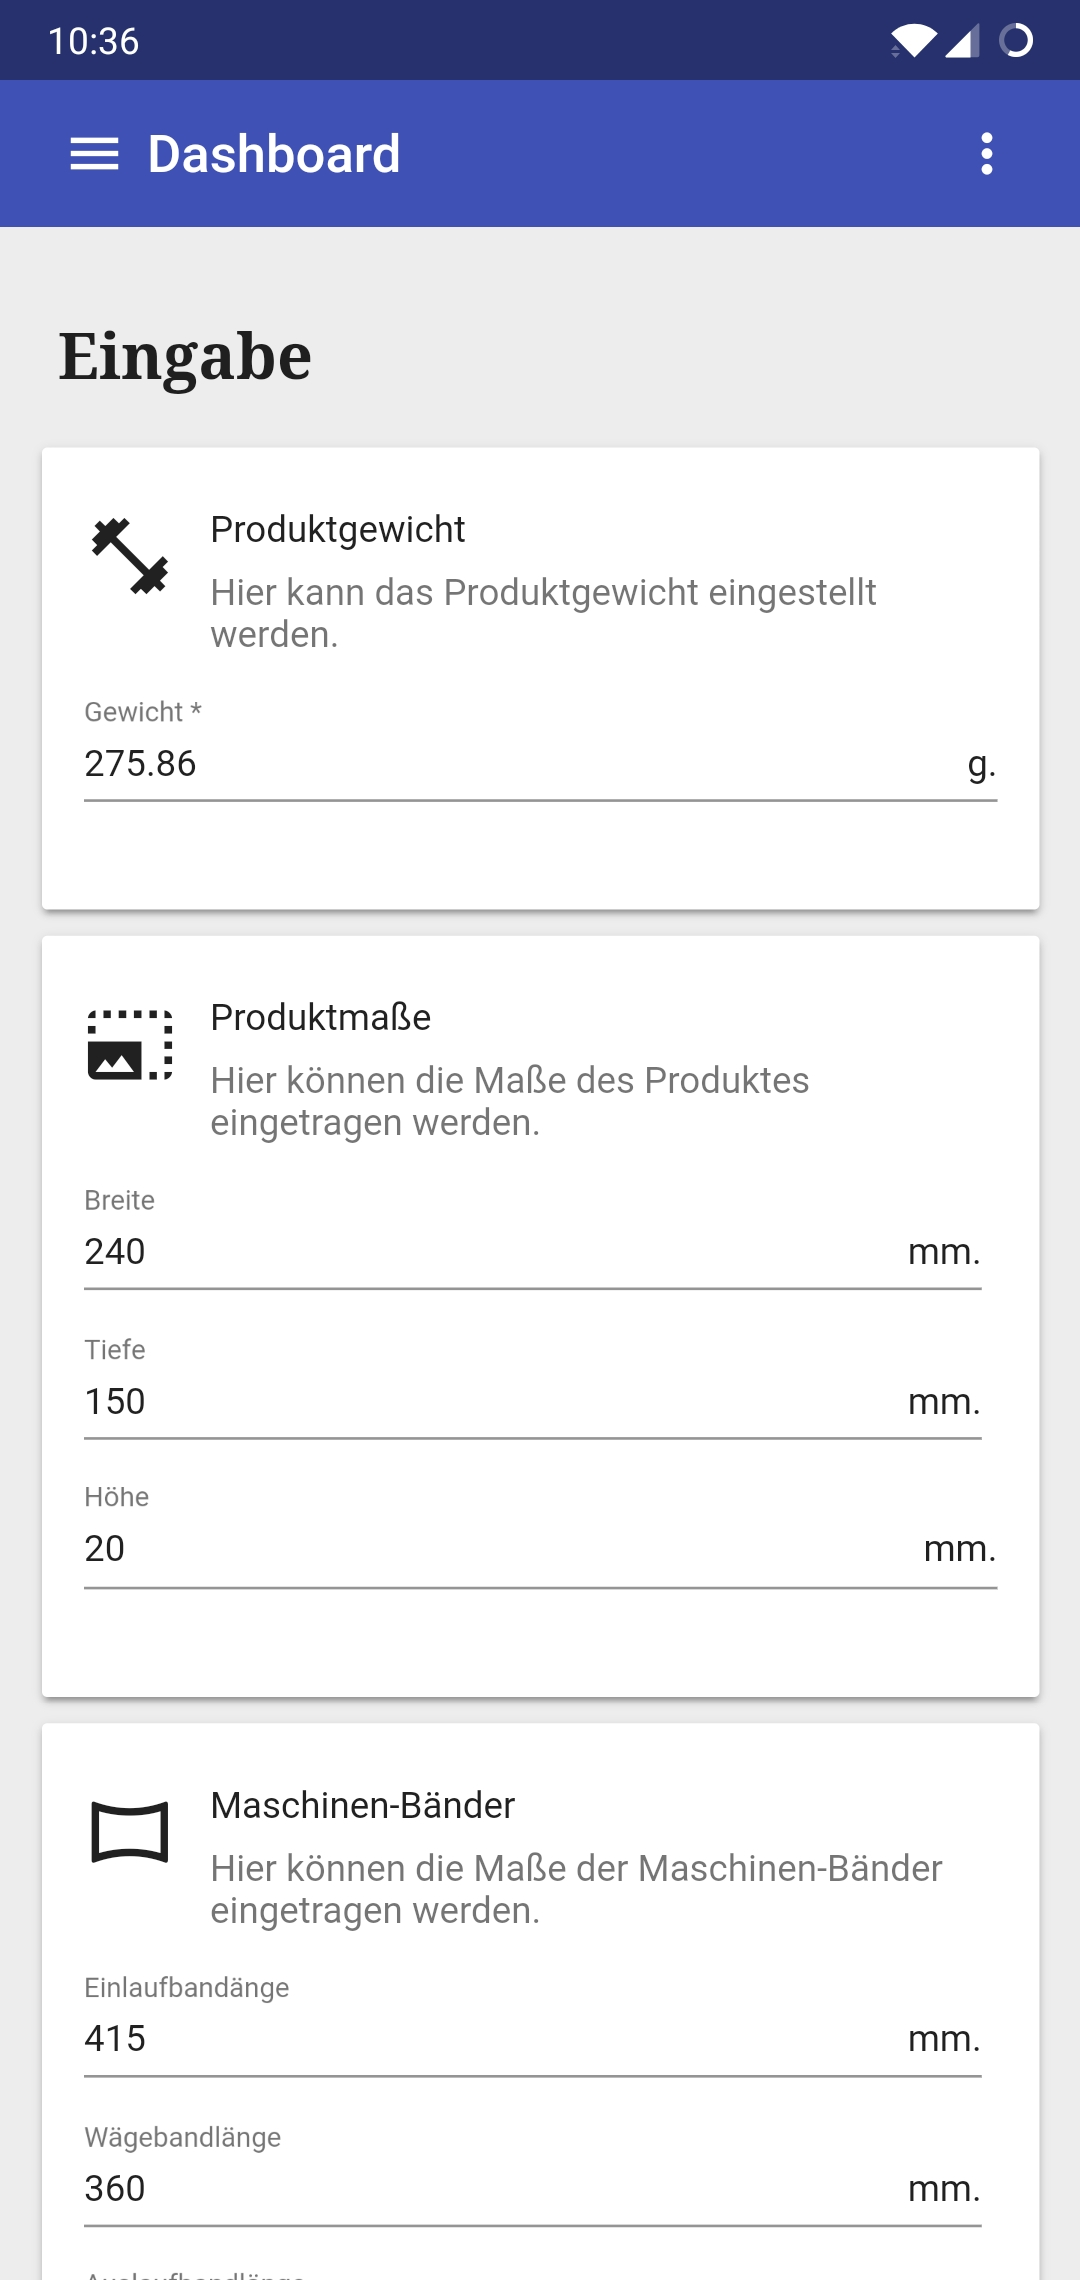
\includegraphics[scale=0.14]{images/kapitel_4/website_smartphone.jpg}
    \caption{Umsetzung der Webseite im responiven Design}
    \label{fig:umsetzung_website_smartphone}
\end{figure}

Bei der Eingabe der einzlenen Formularfelder scrollt man unweigerlich nach unten. Am Ende der Eingabe erscheint dann der
Button zum Erstellen der Vorhersage für die Parameter.

Nach einem Klick auf diesen Button und einer kurzen Ladeanimation erscheint die Ansicht der Ausgabe. Der Nutzer muss
nicht mehr nach unten scrollen.

Auch in der mobilen Version steht die Überschrift für die Ausgabe schon am unteren Rand, damit der Endnutzer weiß, dass
die Informationen unterhalb der Eingabe kommen werden und er nicht unnötig überrascht wird.

\subsubsection{Erweiterungen}
Die Webseite ist fertig entwickelt. Nun kann man sich über Erweiterungen zum Frontend Gedanken machen, die den Endnutzer
bei der Eingabe von Daten unterstützen kann.

Für zahlreiche Erweiterungen, welche im folgenden Behandelt werden, spielt der \textit{Service Worker} eine
entscheidende Rolle. Dieser installiert, definiert über ein Manifest, mittels JavaScript-Technologie einen Proxy
zwischen dem Webbrowser und dem Server.

Mit diesem kann man die Grundlage für Push-Benachrichtigungen, progressive Web-Apps (PWA), offline Modus und komplexer
Cache-Strategie setzen.

Um in der erstellten Angular-Anwendung einen Service Worker zu installieren, benötigt man eine zusätzliche Bibliothek,
welche die interne Konfiguration dafür übernimmt. Diese Bibliothek kann man mittels des folgenden Befehls in die
Anwendung einbauen.

\begin{lstlisting}[caption=Hinzufügen der PWA-Bibliothek, label=ls:umsetzung_angularaddpwa]
    ng add @angular/pwa
\end{lstlisting}

Nun muss man den ServiceWorker in der \textit{angular.json}-Datei aktivieren. Dazu fügt man die Zeile
\textit{\enquote{serviceWorker}: true} in das erste \textit{apps}-Objekt ein.

Mit der Aktivierung der Funktionalität wird beim Bau der Anwendung eine \textit{Angular Service Worker}-Datei mit dem
Namen \textit{ngsw-worker.js} angelegt. Außerdem legt die Bibliothek eine Konfigurationsdatei für den Service Worker mit
dem Namen \textit{ngsw.json} an.

Die erste Datei übernimmt die Installation, das Aktualisieren und das Deinstallieren des Service Workers in dem
durch den Anwender genutzten Browser.

Die zweite Datei kann den Service Worker konfigurieren. So kann man dort zum Beispiel definieren, wie der Service Worker
heißt und welches Icon für ihn angezeigt werden soll.

Die Einrichtung des Service Workers ist damit abgeschlossen. Allerdings funktioniert dieser nur, wenn die
Angular-Anwendung produktiv gebaut (\textit{ng build --prod}) und dann über das Protokoll \textit{https} aufgerufen
wird. Ansonsten verweigern moderne Browser die Nutzung des Service Workers.

Wenn man im Nachgang die Webseite aufruft (mehr dazu im Kapitel~\ref{subsec:toolchain_einrichten} ab
Seite~\pageref{subsec:toolchain_einrichten}), kann man den Service Worker in den \texttt{Entwicklertools} über den
Menüpunkt \texttt{Applikation} und dann \texttt{Service Worker} sehen.

Dort kann man ihn auch als Nutzer zur Aktualisierung zwingen und auch Löschen, falls man bei der Entwicklung
schwerwiegende Fehler eingebaut hat.

\subsubsection{Offline Modus}
Da man im vorangegangenen Kapitel den Service Worker installiert und eingerichtet hat, kann man als nächstes eine der
grundlegensten Funktionen des Service Workers nutzen -- das Caching für einen \textit{offline Modus}.

Damit man diesen umsetzen kann, muss man lediglich die Datei \textit{ngsw.json} anpassen und um alle cachbaren Elemente
erweitern.

In Anhang~\ref{sec:serviceWorkerConfig} auf Seite~\pageref{sec:serviceWorkerConfig} ist die komplette
Konfigurationsdatei angegeben. Diese kann man so nutzen. Nachdem man die Angular-Anwendung wieder im produktiven Modus
gebaut hat, kann man sie aufrufen und alle Elemente werden automatisch im Browser gecached.

Wenn man im Anschluss die Internetverbindung unterbricht (offline Modus oder Netzwerk trennen) und die Webseite
aktualisiert, wird sie trotzdem wie gewünscht angezeigt.

Allerdings kann man in diesem Fall keine Vorhersagen tätigen, da das Backend mit der REST-Schnittstelle nicht abrufbar
ist. Mit einem Klick auf den Button wird ein Fehler ausgegeben, welchen man sich in der Konsole des Browsers ansehen
kann.

Bei dem Fehler handelt es sich um einen \textit{404 Page not found}-Fehler, da die angeforderte Ressource nicht gefunden
werden kann. Dies liegt an der fehlenden Internetverbindung.

Der offline Modus funktioniert auf allen Plattformen in allen gängigen Browsern. So kann man diesen sowohl auf dem
Desktop-Computer nutzen als auch auf dem Smartphone oder einem Tablet.

\subsubsection{Keine offline Abfragen}
Damit man im offline Modus nicht auf den angesprochenen Fehler stößt, wenn man eine Abfrage an das Backend machen
möchte, soll im Weiteren das Frontend selbstständig auf die verschiedenen Modi (online oder offline) reagieren können.

Beispielhaft soll man sich folgendes Szenario vor Augen führen. Ein Endnutzer öffnet bei aktiver Internetverbindung die
Webseite um eine Vorhersage zu tätigen. Damit er die geforderten Eingabeparameter allerdings eingeben kann, muss er zur
betreffenden Maschine und die Daten auslesen.

In dem Raum, in dem sich die Maschine befindet, besteht allerdings keine WLAN Verbindung, worauf die Webseite in den
offline Modus geht. Nachdem der Nutzer die Daten eingetragen hat und eine Vorhersage starten will, würde er einfach
eine Fehlermeldung bekommen, dass das Backend nicht angefragt werden kann.

Eventuell würden seine getätigten Eingaben auch verschwinden, da er versuchen könnte die Webseite neu zu laden.

Um diesem Problem vorzubeugen, soll das Frontent im offline Modus gar keine Anfragen an das Backend machen sondern den
Nutzer informieren, dass es sich aktuell im offline Modus befindet. somit weiß der Nutzer, dass er aktiv nach einer
Internetverbindung suchen muss um fortzufahren.

Um dies zu bewerkstelligen muss man einen Service in die Angular-Anwendung einbauen, welcher immer über den aktuellen
Modus (online oder offline) bescheid weiß und bei einer Änderung allen Komponenten bescheid geben kann.

Mit dem folgenden Befehl kann man einen neuen Service in die Angular-Anwendung einbauen.

\begin{lstlisting}[caption=Hinzufügen eines Services, label=ls:umsetzung_angularaddservice]
    ng generate service network
\end{lstlisting}

Dieser Befehl legt eine Datei mit dem Namen \textit{network.service.ts} an, in der der Service im Weiteren definiert
wird. Die Implementierung der geforderten Funktion ist relativ einfach, da Angular von Haus aus viele Funktionalitäten
mitbringt.

So kann man mit dem in Listing~\ref{ls:umsetzung_angularservicenetwork} auf
Seite~\pageref{ls:umsetzung_angularservicenetwork} definierten Quellcode ein \textit{Observable} anlegen, welches den
aktuellen Netzwerkmodus beinhaltet. Sollte dieser sich ändern, werden alle \textit{Observer} darüber informiert.

\begin{lstlisting}[language=JavaScript, caption=Funktion des Network-Services, label=ls:umsetzung_angularservicenetwork]
    public isConnected = true;

    constructor(private connectionService: ConnectionService) {
        this.connectionService.monitor().subscribe(isConnected => {
            this.isConnected = isConnected;
        })
    }
\end{lstlisting}

Die vierte Zeile \textit{subscribed} sich auf einen Angular internen \textit{Observable}, welcher die Information
beinhaltet, ob eine Internetverbindung aktuell besteht oder nicht. Die Information, welche aus dem internen Service
kommt, wird in der lokalen Variable \textit{isConnected} gespeichert. Diese Speicherung führt man in Zeile fünf durch.

Die Varibale, die den aktuellen Modus der Internetverbindung hält, definiert man am Besten global in dem Service und
damit weit oben in der Datei. Hier symbolisiert durch die Zeile eins.

Anschließend kann man bei jeder Anfrage an das Backend das in Listing~\ref{ls:umsetzung_angularchecknetwork} auf
Seite~\pageref{ls:umsetzung_angularchecknetwork} definierte If-Statement nutzen, um zu überprüfen ob aktuell eine
Internetverbindung vorliegt oder nicht. Falls nicht, sollte man den Nutzer über einen gut sichtbaren Hinweis darüber
informieren, dass aktuell keine Abfrage möglich ist.

\begin{lstlisting}[language=JavaScript, caption=Überprüfung ob eine Internetverbindung vorliegt, label=ls:umsetzung_angularchecknetwork]
    if (this.networkService.isConnected) {
        ...
    } else {
        ...
    }
\end{lstlisting}

In der Zeile zwei definiert man den Programmteil, welcher bei aktiver Internetverbindung ausgeführt wird. Also zum
Beispiel die Abfrage an das Backend. In der vierten Zeile kann man dann die Meldung ausgeben die angezeigt wird, wenn
der Nutzer über keine Internetverbindung verfügt.

Auch wäre es möglich einen dauerhaften Hinweis einzublenden, wenn keine Internetverbindung vorliegt. Dies müsste man
dann in der \textit{app.component.ts} Datei global machen. Dabei ist entscheidend, dass das nicht mit einem If-Statement
möglich ist. Man muss dies mit einem Observer lösen.

Mit einer Snackbar\footnote{https://material.angular.io/components/snack-bar/overview} kann man den entsprechenden
Hinweis optimal anzeigen und positionieren lassen. Dabei handelt es sich um eine Komponente des Material-Deisgns.

\subsubsection{Toolchain einrichten}
\label{subsec:toolchain_einrichten}
Im letzten Schritt zur Entwicklung des Frontends muss man die Toolchain einrichten, damit man den geschriebenen
Quellcode auch automatisiert in einem Cloud Foundry Container in der Cloud installieren kann.

Dabei ist die Konfiguration der Pipeline nicht ganz so einfach wie die beim Erstellen des TensorFlow-Containers, da man
die Angular-Anwendung bauen muss, bevor man sie in den Container schieben kann.

Auch ist der gebaute Quellcode in einem anderen Ordner als der Teil, welchen man in das Git-Repository lädt. So sind
nacheinander wenige Schritte notwendig, damit man die gebaute Anwendung auch richtig in den Container schieben kann.

In einem ersten Schritt muss man die Toolchain jedoch erst anlegen. Dies kann man über das Cloud Foundry Dashboard der
IBM Cloud machen. Dazu geht man auf das IBM Cloud Dashboard und klickt auf die vorher angelegte Runtime der
Angular-Anwendung.

Nun öffnet sich das Cloud Foundry Dashboard über das man am unteren Bereich auf den Button \texttt{Aktivieren} in der
Box \texttt{Continous Delivery} klicken kann. Genau wie in Kapitel~\ref{sub:tollchain_einrichten} auf
Seite~\pageref{sub:tollchain_einrichten} gelangt man damit auf die Konfigurationsseite der Toolchain.

Jetzt muss man einen Namen für die Toolchain definieren und die Region auswählen. Da auch hier die Standartkonfiguration
ausreicht, kann man die Toolchain mit einem Klick auf den Button \texttt{Erstellen} einrichten.

Nach einem kurzen Ladevorgang ist die Toolchain eingerichtet und mit einem leeren Git-Repository vorkonfiguriert.
Aktuell ist lediglich die \textit{Delivery Pipeline} interessant, da man hier die Installation der Angular-Anwendung
spezifizieren muss.

In der aktuellen Konfiguration sind drei \textit{Stages} eingerichtet. Diese muss man nun um zwei weitere Ergänzen,
sodass es eine \textit{Build-}, eine \textit{Angular build-}, eine \textit{Copy files-}, eine \textit{Test-} und eine
\textit{Deploy-}Stage gibt.

Der Aufbau der Toolchain ist in der Abbildung~\ref{fig:umsetzung_toolchain_pipeline_frontend} auf der
Seite~\pageref{fig:umsetzung_toolchain_pipeline_frontend} zu sehen.

\begin{figure}[h]
    \centering
    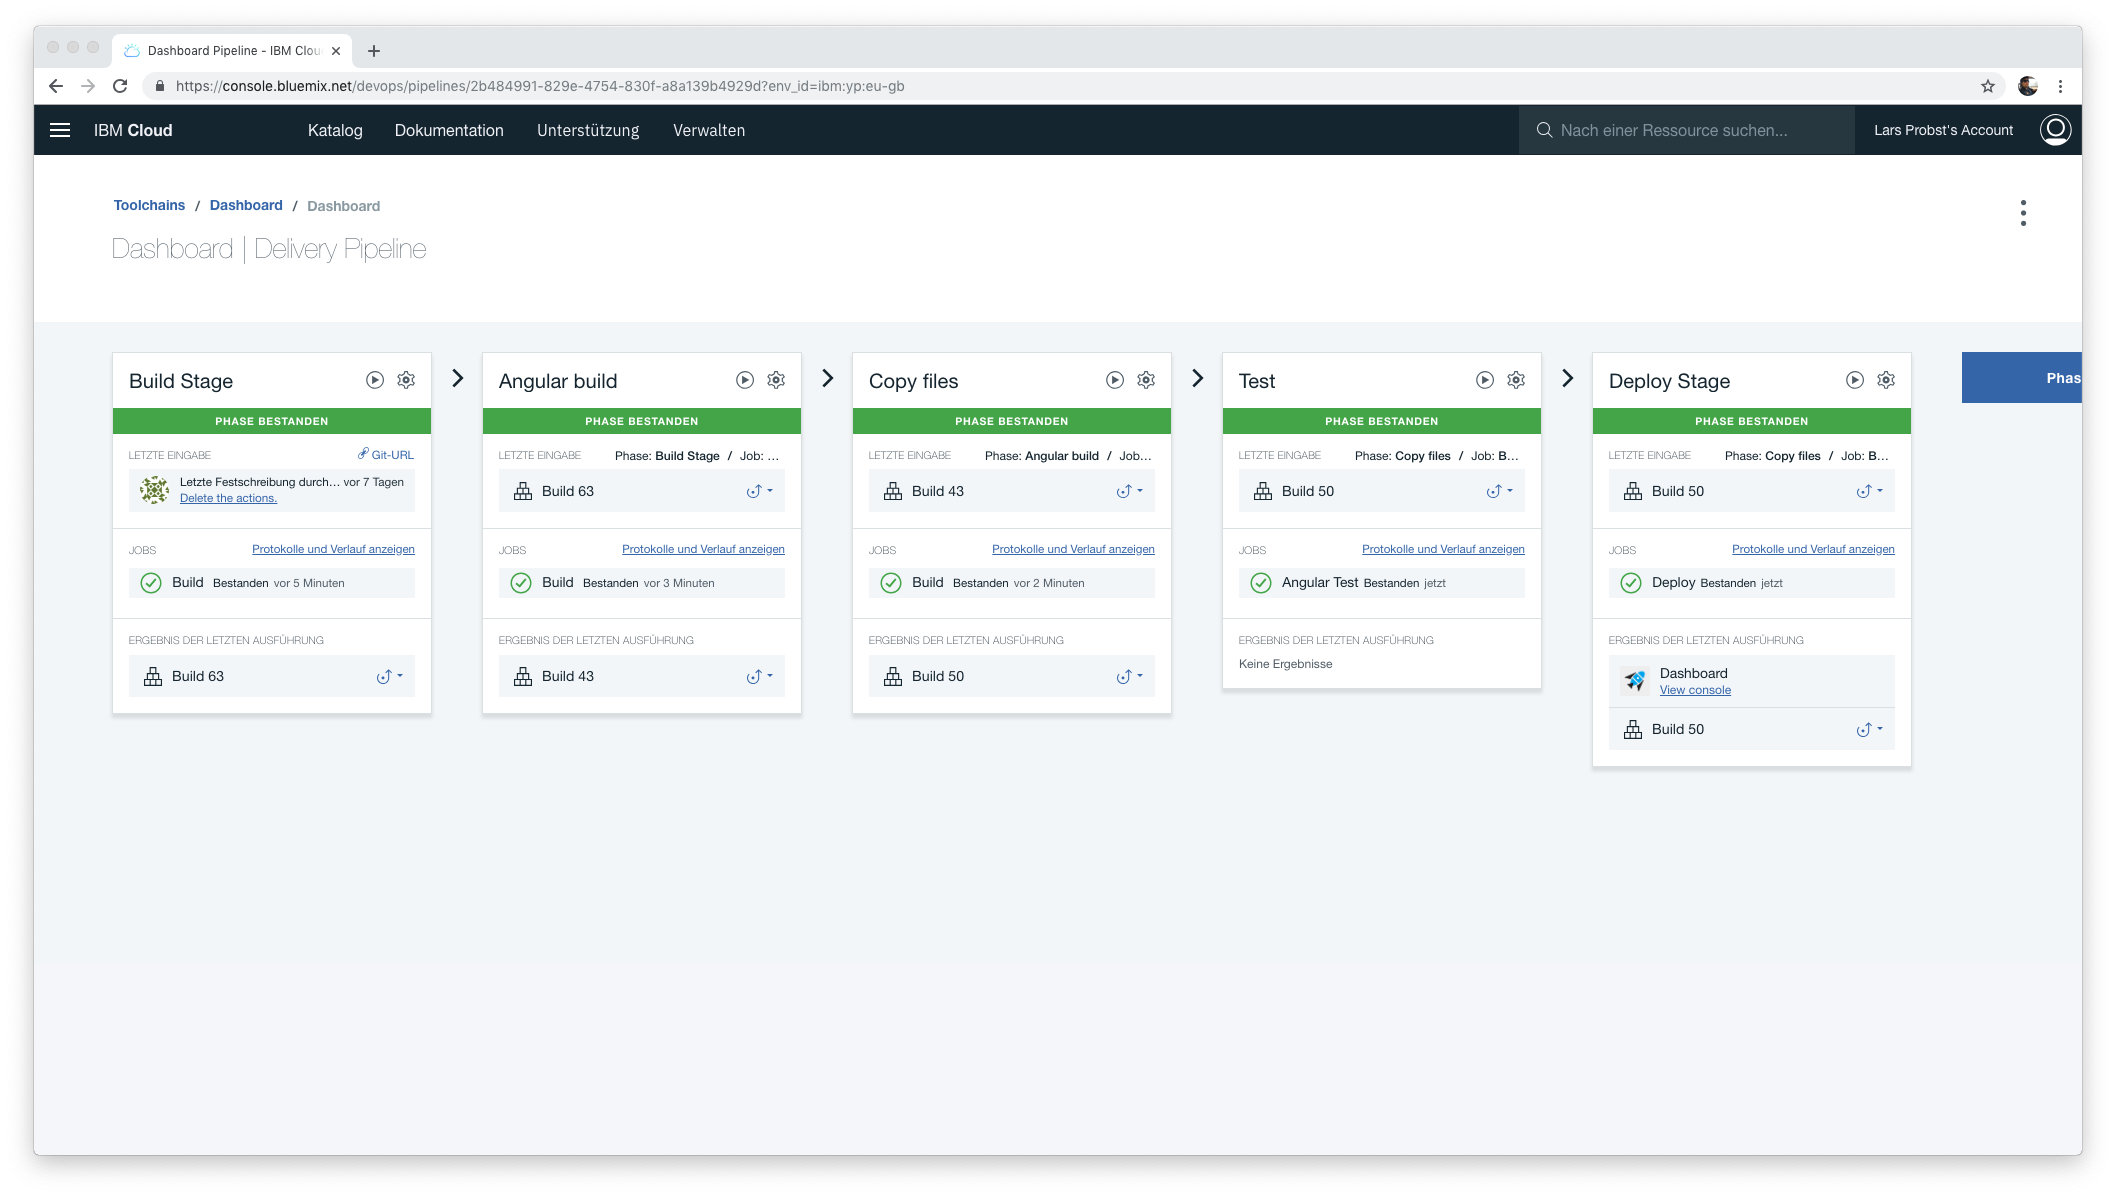
\includegraphics[width=\textwidth]{images/kapitel_4/toolchain_pipeline.png}
    \caption{Übersicht der Toolchain-Konfiguration}
    \label{fig:umsetzung_toolchain_pipeline_frontend}
\end{figure}

Die \textbf{Build Stage} entspricht der Standard Build Stage der Toolchain-Konfiguration und man kann diese unverändert
beibehalten. Sie ist für das Laden des Quellcodes aus dem Git-Repository zuständig und wird immer dann ausgeführt,
sobald ein \textit{commit} in das Repository \textit{gepushed} ist.

In der \textbf{Angular Build} Stage wird die Angular-Anwendung mittels des Befehls \textit{ng build --prod} gebaut. Dies
ist wichtig, damit ein \texttt{dist}-Ordner entsteht, welcher alle kaskadierten CSS"~ und HTML-Dateien enthält. Auch
werden CSS"~ oder HTML-Platzhalter ausgetauscht und die Angular-Anwendung betriebsbereit geschaltet. Dies ist zum
Beispiel auch für den offline Modus und den Service Worker entscheidend.

Die nächste Stage, \textbf{Copy files}, kümmert sich um das Kopieren der Inhalte aus dem \texttt{dist}-Ordner. Später
soll in dem Cloud Foundry Container nicht der Quellcode laufen, welcher in das Git-Repository geladen wurde. Sondern
der, welcher mittels der vorangegangenen Stage durch die Angular-CLI gebaut wurde. Darum muss man, bis auf den Inhalt
des \texttt{dist}-Ordners, alle Dateien und Ordner löschen.

Um die Funktionalität einer Anwendung stetig gewährleisten zu können sollte man Tests für alle Funktionen bereitstellen.
Die \textbf{Test}-Stage kümmert sich um die Ausführung der Tests. Nur wenn alle erfolgreich durchlaufen, wird der Inhalt
an das Deployment übergeben um den Cloud Foundry Container zu befüllen.

Die definierten Tests in der Angular-Anwendung werden über \textit{ng test} ausgeführt. Dieser Kommandozeilenaufruf
startet einen Headless-Browser, welcher die einzelnen Testschritte anschließend durchgeht.

Die letzte Stage, \textbf{Deploy Stage}, ist die Stadard-Stage der Toolchain für das Installieren der Anwendung. Auch
diese kann man aus der Ursprungskonfiguration übernehmen.

Somit ist die Toolchain fertig konfiguriert und man kann den Quellcode in das Git-Repository laden um die Toolchain zu
starten. Nach wenigen Minuten ist die Anwendung in einem Cloud Foundry Container über ihre Domain im Browser aufrufbar
und man kann damit beginnen Anfragen an das Backend zu schicken.

Da man in Kapitel~\ref{subsec:apiconnect} auf Seite~\pageref{subsec:apiconnect} den API Connect Service mit den beiden
Backends verbunden hat, kann man nun aus dem Frontend heraus Anfragen an diese stellen und die Vorhergesagten Parameter
werden angezeigt.

Im Weiteren kann man damit beginnen das Frontend in die Smartphone-Apps einzubauen, da es über eine Domain und ein
valides SSL-Zertifikat verfügt.

Nur damit ist es Möglich die Webseite in ein WebViewer zu laden und dem Endnutzer anzuzeigen. Auch für die
Funktion des Service Workers und des offline Modus ist ein SSL-Zertifikat und eine Domain essentiell.

\subsection{Smartphone-Apps}
Da das Frontend (Dashboard) nun fertig entwickelt und über eine Domain aufrufbar ist, kann man es im nächsten Schritt
für die Umsetzung der Smartphone-Apps nutzen.

Die Umsetzung der Smartphone-Apps erfolgt auf Basis von Android und iOS. Dies hat den Vorteil, dass ein größerer
potentieller Kundenkreis gewonnen werden kann, da diese beiden Systeme die mobilen Betriebssysteme
dominieren~\cite{online_umsetzung_mobileos}.

In den zwei folgenden Kapiteln werden die Umsetzungen für die beiden Betriebssysteme erläutert. Insbesondere wird auf
die technischen Unterschiede der Systeme eingegangen um ein WebView-Layout zu nutzen.

Die Smartphone-Apps kann man anschließend in einem Emulator lokal auf dem Entwicklungsrechner testen um Fehler in der
gebauten Version auszuschließen.

\subsubsection{Android}
Für die Erstellung einer Android-App benötigt man die Android Studio IDE. Diese kann man kostenlos auf der
Developper-Seite\footnote{https://developer.android.com/studio} von Google herunterladen. Die Anwendung steht für
Windows, Linux und macOS zur Verfügung. Android Studio basiert auf der Community-Edition von IntelliJ und ist kostenlos.

Für die Verwendung von Android Studio benötigt man eine installierte Version des Java-JRE und das Java-JDK. Die JRE
benötigt man für das Ausführen der IDE und die JDK für das Bauen des Quellcodes und der APK-Datei. Die aktuellste
Version von Java wird für die Nutzung empfohlen. Dies ist zur Zeit die Version 9.

Nachdem man die IDE und gegebenenfalls Java installiert hat, kann man Android Studio zum ersten Mal starten. Beim ersten
Aufruf muss man das Android-SDK herunterladen sowie einen Emulator konfigurieren. Dabei sollte man jeweils die neuesten
Versionen auswählen. Mit dem Emulator kann man die App nachher auf dem Rechner starten und live testen.

Es ist möglich eine Android-App mittels \textit{Java}, \textit{Kotlin} und \textit{C\texttt{++}} zu entwicklen. Im
folgenden wird auf die Verwendung von \textbf{Kotlin} zurückgegriffen, da es den Quellcode sehr schlank macht und
dadurch eine bessere Übersicht bietet.

Im nächsten Schritt muss man ein neues Projekt anlegen. Dazu wird zum Beispiel der Name \textit{Dashboard} ausgewählt.
Also Projekttyp kann man ein leeres Android-Projekt auswählen. Dadurch werden keine Klassen oder Layouts angelegt.

Die Android-App muss im Ordner \texttt{/res/layout} ein Layout besitzen, welches als Root-Element ein
\textit{CoordinatorLayout} enthält und als Kind-Element ein einzelnes, natives WebView-Layout. Diesem Layout wird eine
ID zugeteilt, damit man es aus der Kotlin-Klasse heraus eindeutig identifizieren kann.

Nun kann man im \texttt{/src}-Ordner zwei Kotlin-Klassen anlegen. Eine für die MainActivity, welche die Hauptroutine der
Anwendung enthält. Die andere ist für den SplashScreen, welcher beim Start der App angezeigt wird. Der Splashscreen
zeigt das Bosch-Logo und wechselt nach ein paar Sekunden in die Hauptroutine um den WebViewer darzustellen.

Die MainActivity enthält eine unveränderliche Variable vom Typ \textit{Text} um die URL des Frontends zu definieren. In
der \textit{onCreate}-Methode kann man dann das WebViewer-Layout konfigurieren, damit die Nutzung von JavaScript möglich
ist.

Das WebView-Layout, welches von der \textit{Android-WebKit} Klasse erbt, kümmert sich anschließend um das Laden der
Webseite, die Darstellung und die Interaktion des Nutzers damit.

Wenn man Funktionen der \textit{WebViewClient} überschreibt kann man das Verhalten des WebViews anpassen. So kann man
beispielsweise Einfluss auf den Titel oder andere HTML-Elemente nehmen.

In den beiden Ordnern \texttt{/res/values} und \texttt{/res/values-v21} kann man Farben und Styles definieren. Im Ordner
mit der Endung \textit{v21} kann man Styles und Farben definieren, welche erst ab der Android in der Version 21 genutzt
werden.

Die Datei"~ und Ordnerstruktur der Android-Anwendung kann man in der Abbildung~\ref{fig:umsetzung_android_folder} auf
Seite~\pageref{fig:umsetzung_android_folder} einsehen.

\begin{figure}[h]
    \centering
    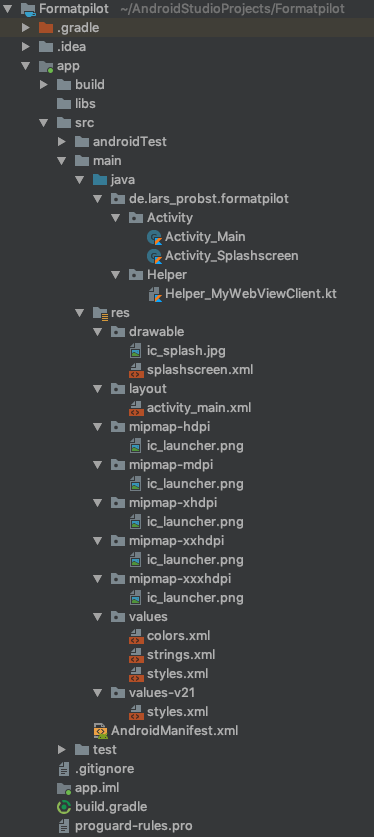
\includegraphics[scale=0.3]{images/kapitel_4/android_folder.png}
    \caption{Ordner und Dateien in Android Studio}
    \label{fig:umsetzung_android_folder}
\end{figure}

Der Ordner \texttt{/res/drawable} enthält das Splashscreen-Logo, also das Bosch-Logo, und die Konfiguration für den
Hintergrund des Splashscreens.

Die \textit{Manifest.xml}-Datei ist Elementar für jede Android-Anwendung. Über diese kann man die Informationen und
Konfigurationen der gesamten App anpassen.

Zum Beispiel ist es dort möglich zu definieren, welche Activity beim Start der Anwendung geladen werden soll. Weitere
Informationen zu dieser Manifest Datei sind in der
Android-Developer-Seite\footnote{https://developer.android.com/guide/topics/manifest/manifest-intro} verfügbar.

In der Abbildung~\ref{fig:umsetzung_android_app} auf Seite~\pageref{fig:umsetzung_android_app} ist die fertig
entwickelte Android-App in einem Smartphone-Emulator sichtbar.

\begin{figure}[h]
    \centering
    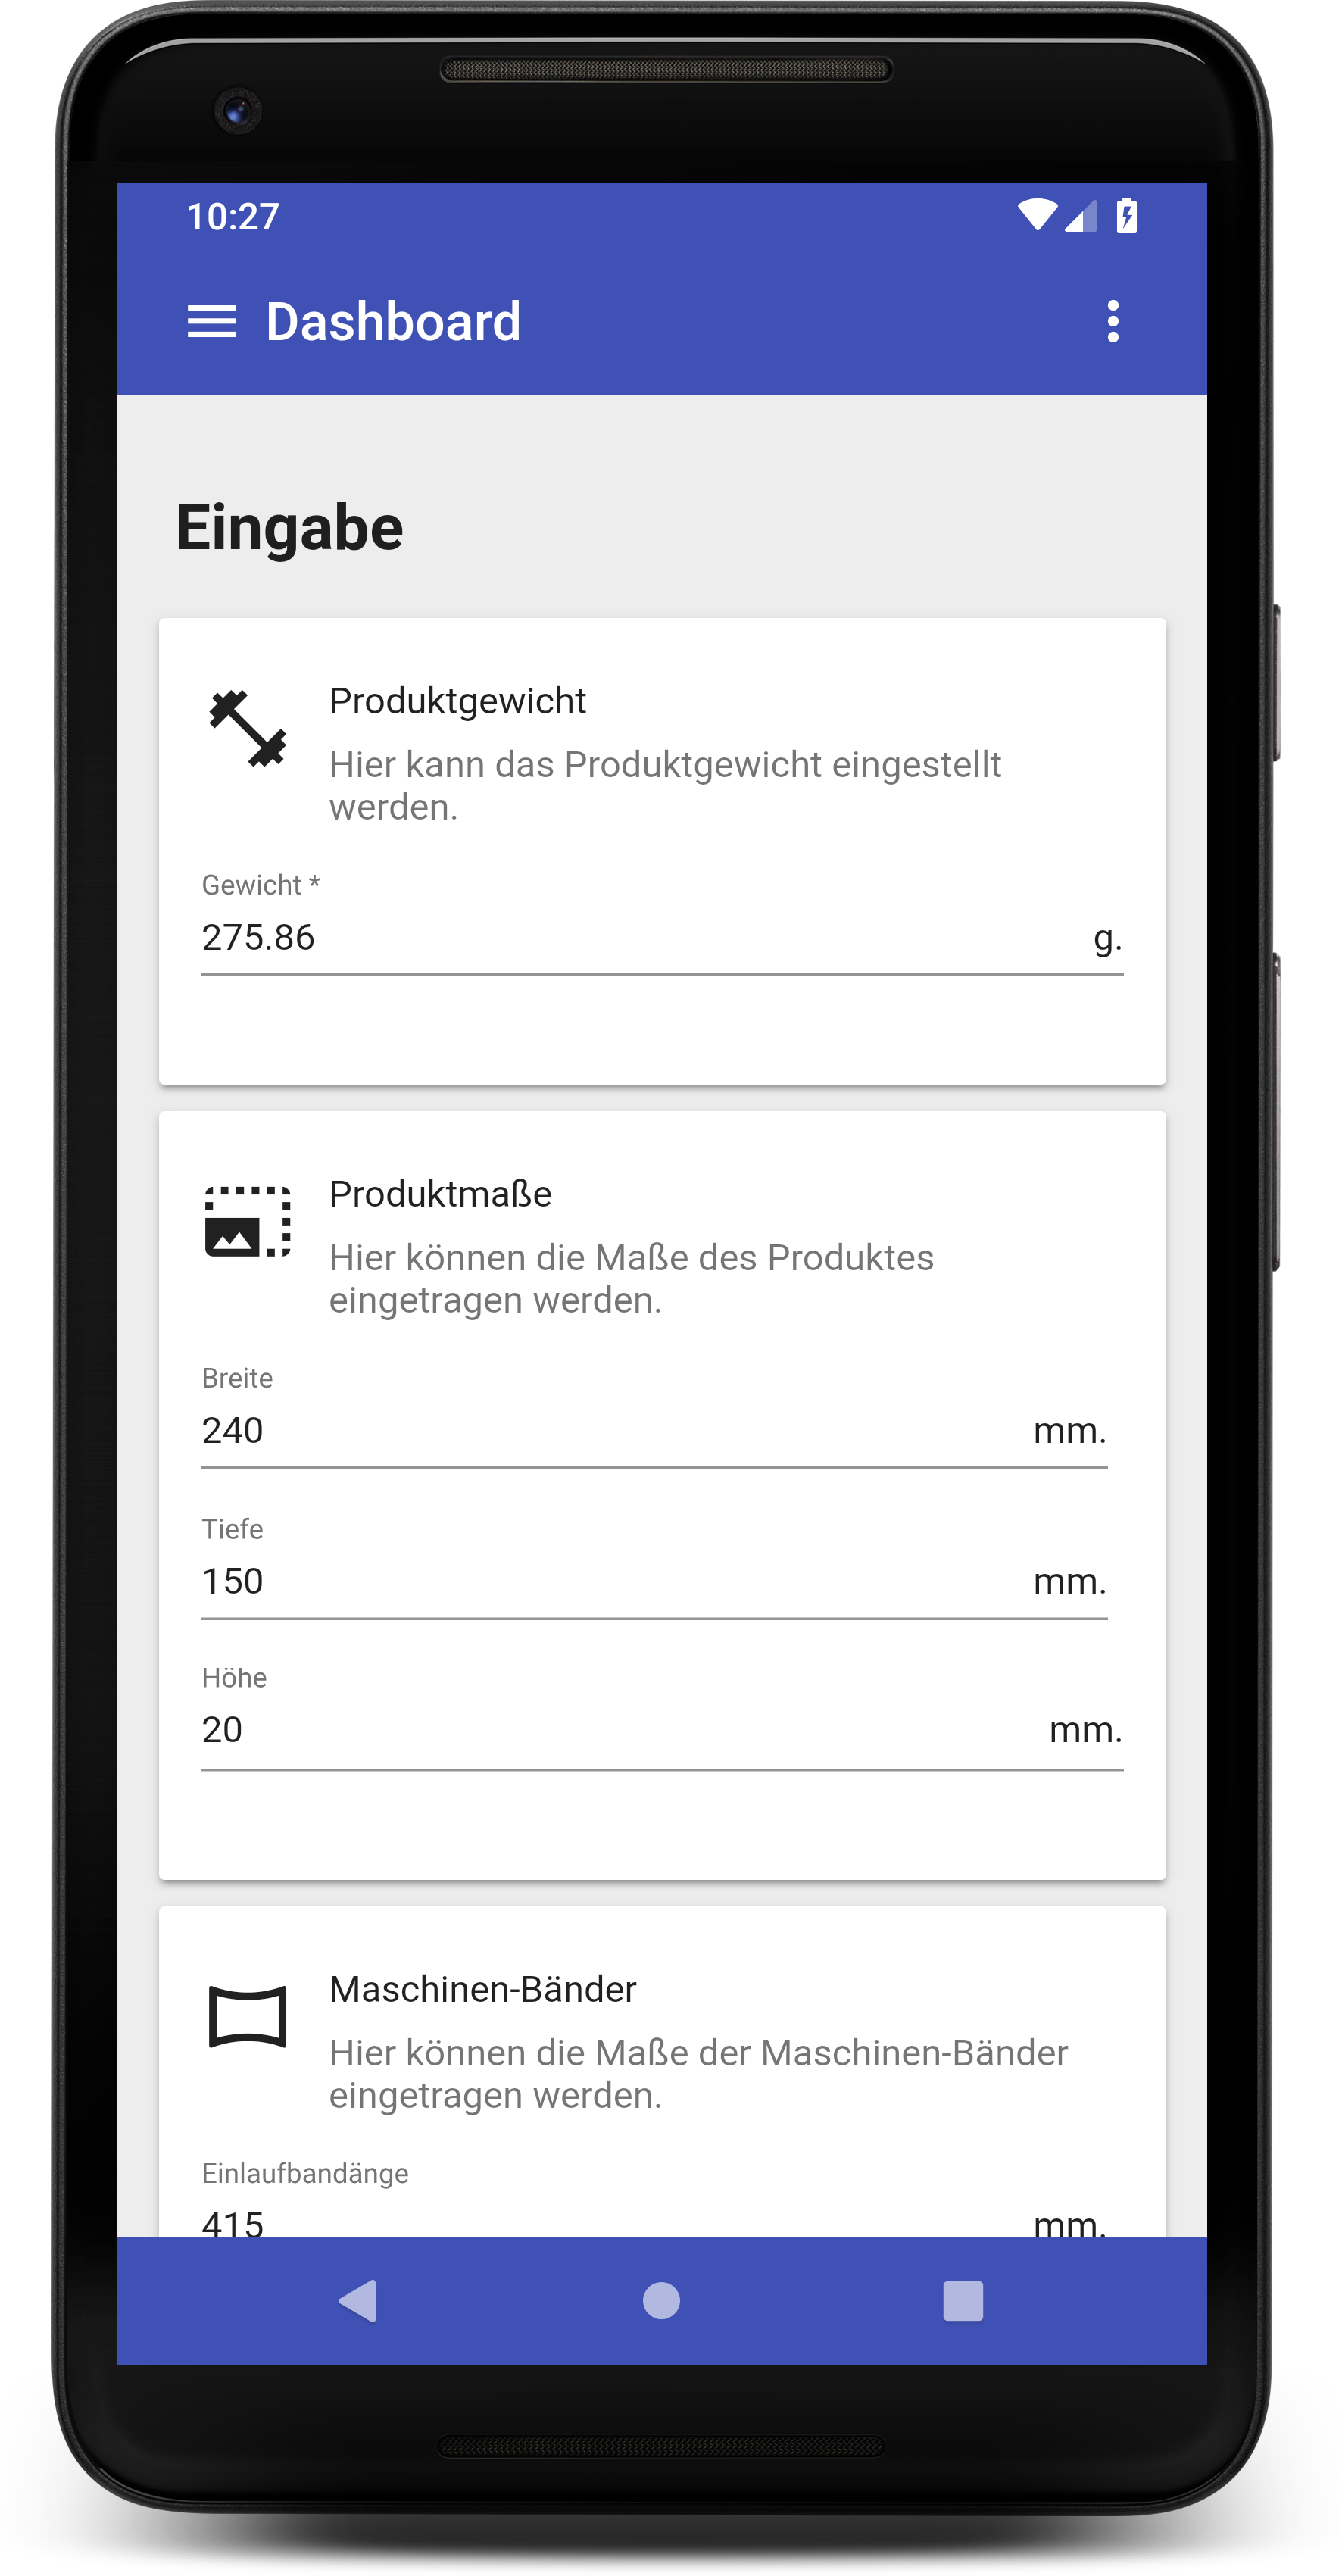
\includegraphics[scale=0.095]{images/kapitel_4/android_app.png}
    \caption{Android-App im Smartphone-Emulator}
    \label{fig:umsetzung_android_app}
\end{figure}

In dieser Abbildung ist leicht zu sehen, dass die Antroid-Styles direkten Einfluss auf die Darstellung der Menüpunkte
(am unteren Rand) und die Farbe der Toolbar haben. Beide werden in der selben Farbe wie der Header im Web-Frontend
dargestellt.

Die Android-App ist an dieser Stelle fertig entwickelt und man kann sie in eine APK-Datei exportieren. Dazu muss man
eine \textit{Signing-Datei} erstellen mit welcher es dann möglich ist, die Anwendung auch in den Play-Store zu laden.

Alternativ kann man die exportierte Android Package-Datei (kurz APK) auch auf einem echten Smartphone oder Tablet
installieren um sie unter echten Bedingungen zu testen.

\subsubsection{iOS}
Um eine App für iOS Geräte zu entwickeln, benötigt man die kostenlose IDE Xcode von Apple. Diese steht lediglich für
macOS-Geräte zur Verfügung und man kann sie nur im
App-Store\footnote{https://itunes.apple.com/de/app/xcode/id497799835} herunterladen.

Somit kann man iOS Apps lediglich unter macOS und Xcode schreiben, kompilieren und testen. Dies stellt eine sehr große
Einschränkung dar.

Nach der erfolgreichen Installation kann man in Xcode anschließend ein neues Projekt anlegen. Die Art des Projektes ist
\textit{SingleViewApp} und den Namen kann auf \textit{Dashboard} setzen.

In der Abbildung~\ref{fig:umsetzung_ios_ide} auf Seite~\pageref{fig:umsetzung_ios_ide} ist das erstellte Projekt in
Xcode zu sehen. Der lokale Emulator und die verschiedenen SDKs sind automatisch mitinstalliert.

\begin{figure}[h]
    \centering
    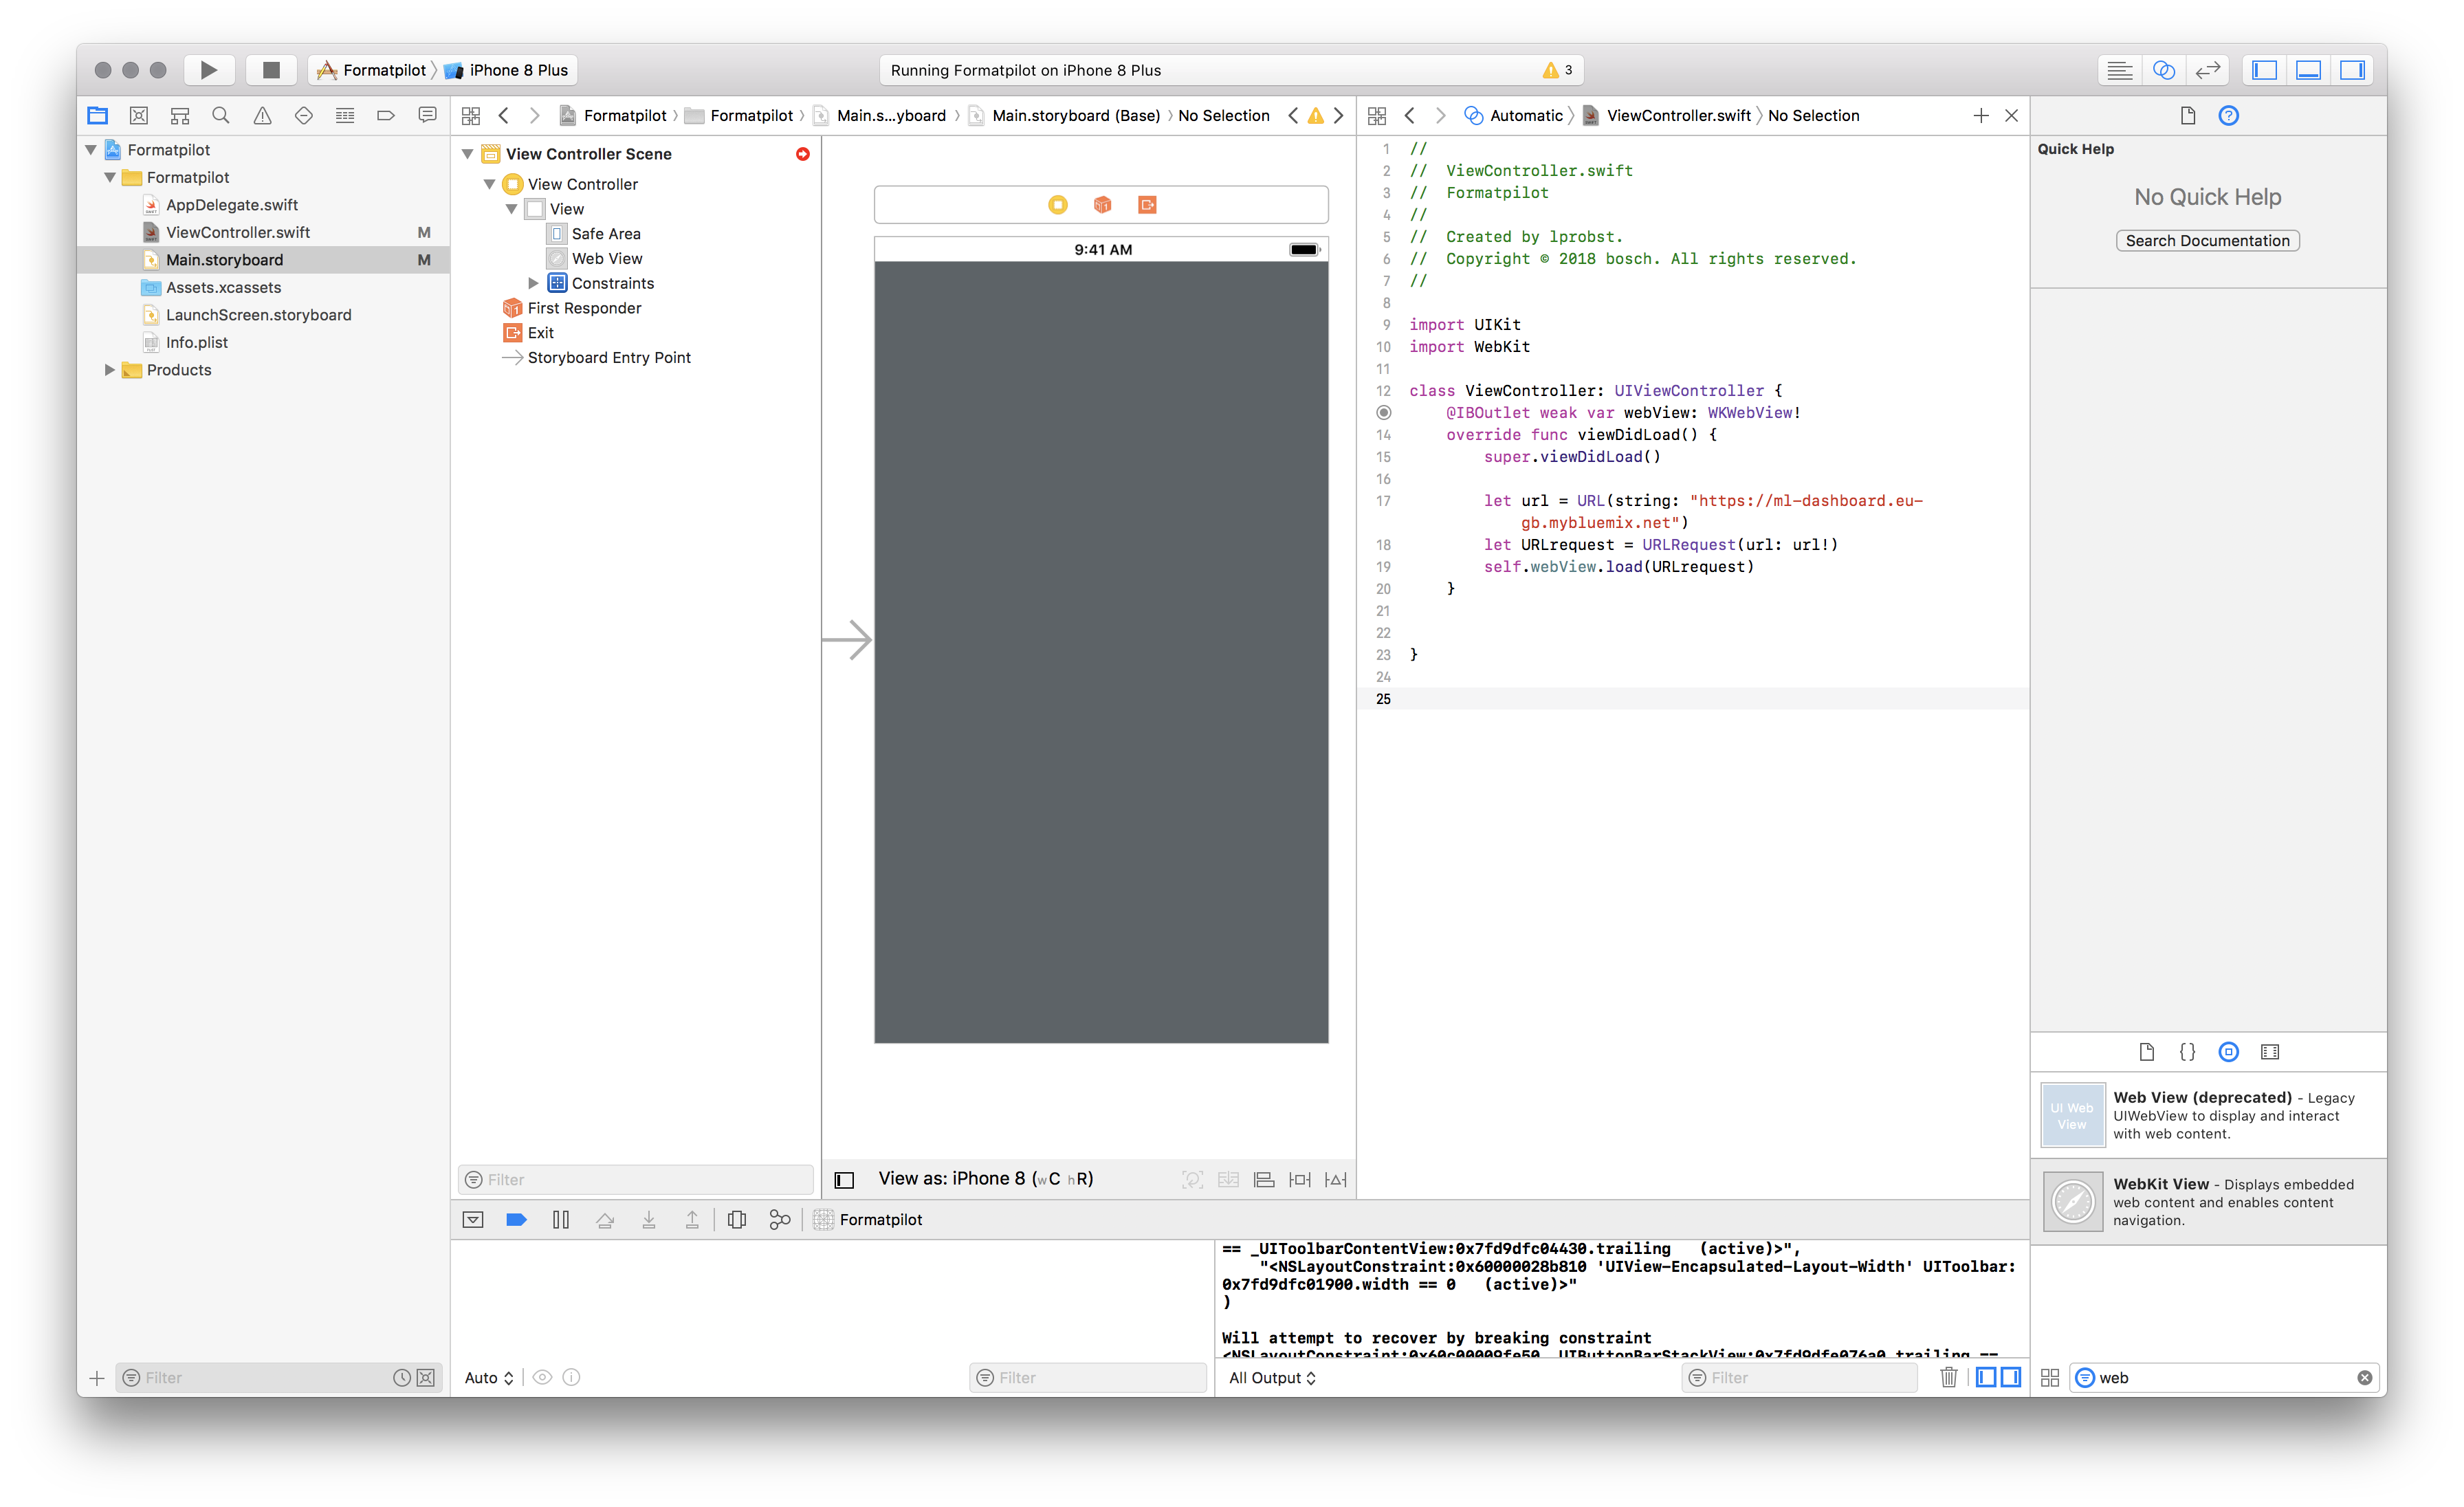
\includegraphics[width=\textwidth]{images/kapitel_4/ios_ide.png}
    \caption{Übersicht von Xcode}
    \label{fig:umsetzung_ios_ide}
\end{figure}

Bei den beiden \texttt{.swift}-Dateien handelt es sich um die ausführbaren Klassen innerhalb der Anwendung. Ihn ihnen
kann man die Logik entwickeln, die für die Anwendung notwendig sind.

Dabei übergibt man in der \textit{ViewController}-Datei die genutzte View und konfiguriert diese. Wie in der Abbildung
zu sehen ist das genutzte View ein WebView-Layout, dem man die URL übergibt.

In der Datei \textit{AppDelegate} definiert man den Lifecycle der Anwendung. So kann man dort zum Beispiel festlegen,
dass der genutzte Controller das \textit{LaunchScreen}-Storyboard zugeteilt bekommt.

Generell sind die \texttt{.storyboard}-Dateien für die Darstellung der einzelnen Seiten und Menüpunkte zuständig. Davon
benötigt man lediglich eine, welche das Web-Frontend darstellt.

Die iOS-App erhält in dieser Version keine eigene View mit einem Splashscreen und zeigt nach dem Start direkt das
WebView-Layout an.

Zum Schluss benötigt man die \texttt{.plist}-Datei, die die Konfiguration der Anwendung übernimmt. Sie ist ähnlich der
Android-Manifest-Datei und kümmert sich um grundlegende Konfigurationen.

In der Abbildung~\ref{fig:umsetzung_ios_folder} auf Seite~\pageref{fig:umsetzung_ios_folder} ist die Übersicht der
Datei"~ und Ordnerstruktur in Xcode abgebildet. Dort sind alle benötigten Dateien für das Projekt zu sehen.

\begin{figure}[h]
    \centering
    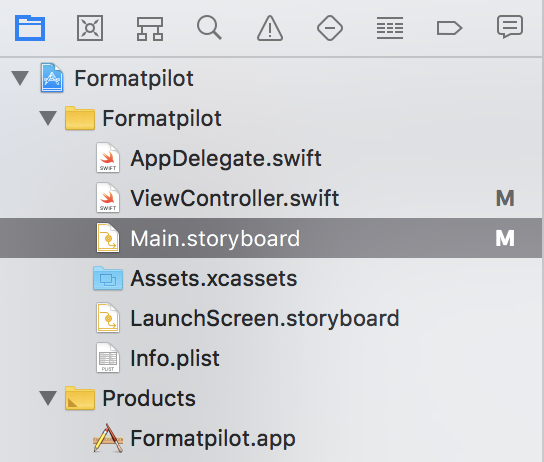
\includegraphics[scale=0.6]{images/kapitel_4/ios_folder.png}
    \caption{Ordner und Dateien in Xcode}
    \label{fig:umsetzung_ios_folder}
\end{figure}

Die Plist-Datei (Property List Files) beinhaltet die Konfiguration der Anwendung. So kann man hier zum Beispiel
einstellen, ab welcher iOS-Version die App zur Verfügung steht oder ob es beispielsweise einschränkungen in der
Ausrichtung des Bildschirmes gibt.

Außerdem definiert man hier den Namen der Anwendung und das verwendete Icon das auf dem Home-Screen angezeigt werden
soll.

Anschließend muss man im Storyboard, also der View, ein WebView-Layout anlegen. Dies kann man mit der Programmiersprache
Swift dann ansprechen und konfigurieren. Ähnlich der Android-App kann man Informationen wie Domain oder Anzeigegröße
übergeben und das Layout kümmert sich selbstständig um das Laden, das Darstellen und die Interaktion zwischen Nutzer und
Webseite.

Mit einem Klick auf \texttt{Run} (der kleine schwarze Play-Button) in Xcode, kann man den zu nutzenden Emulator
auswählen, welcher die Anwendung starten soll.

Nach wenigen Augenblicken ist der Emulator gestartet und zeigt die entwickelte App an. Man kann diese so nutzen, als
würde man sie auf einem echten Smartphone starten. Das Frontend sollte nach wenigen Sekunden ladezeit vollflächig
angezeigt sein.

In der Abbildung~\ref{fig:umsetzung_ios_app} auf Seite~\pageref{fig:umsetzung_ios_app} ist die Anwendung im Smartphone
Emulator mit der neuesten iOS Version zu sehen.

\begin{figure}[h]
    \centering
    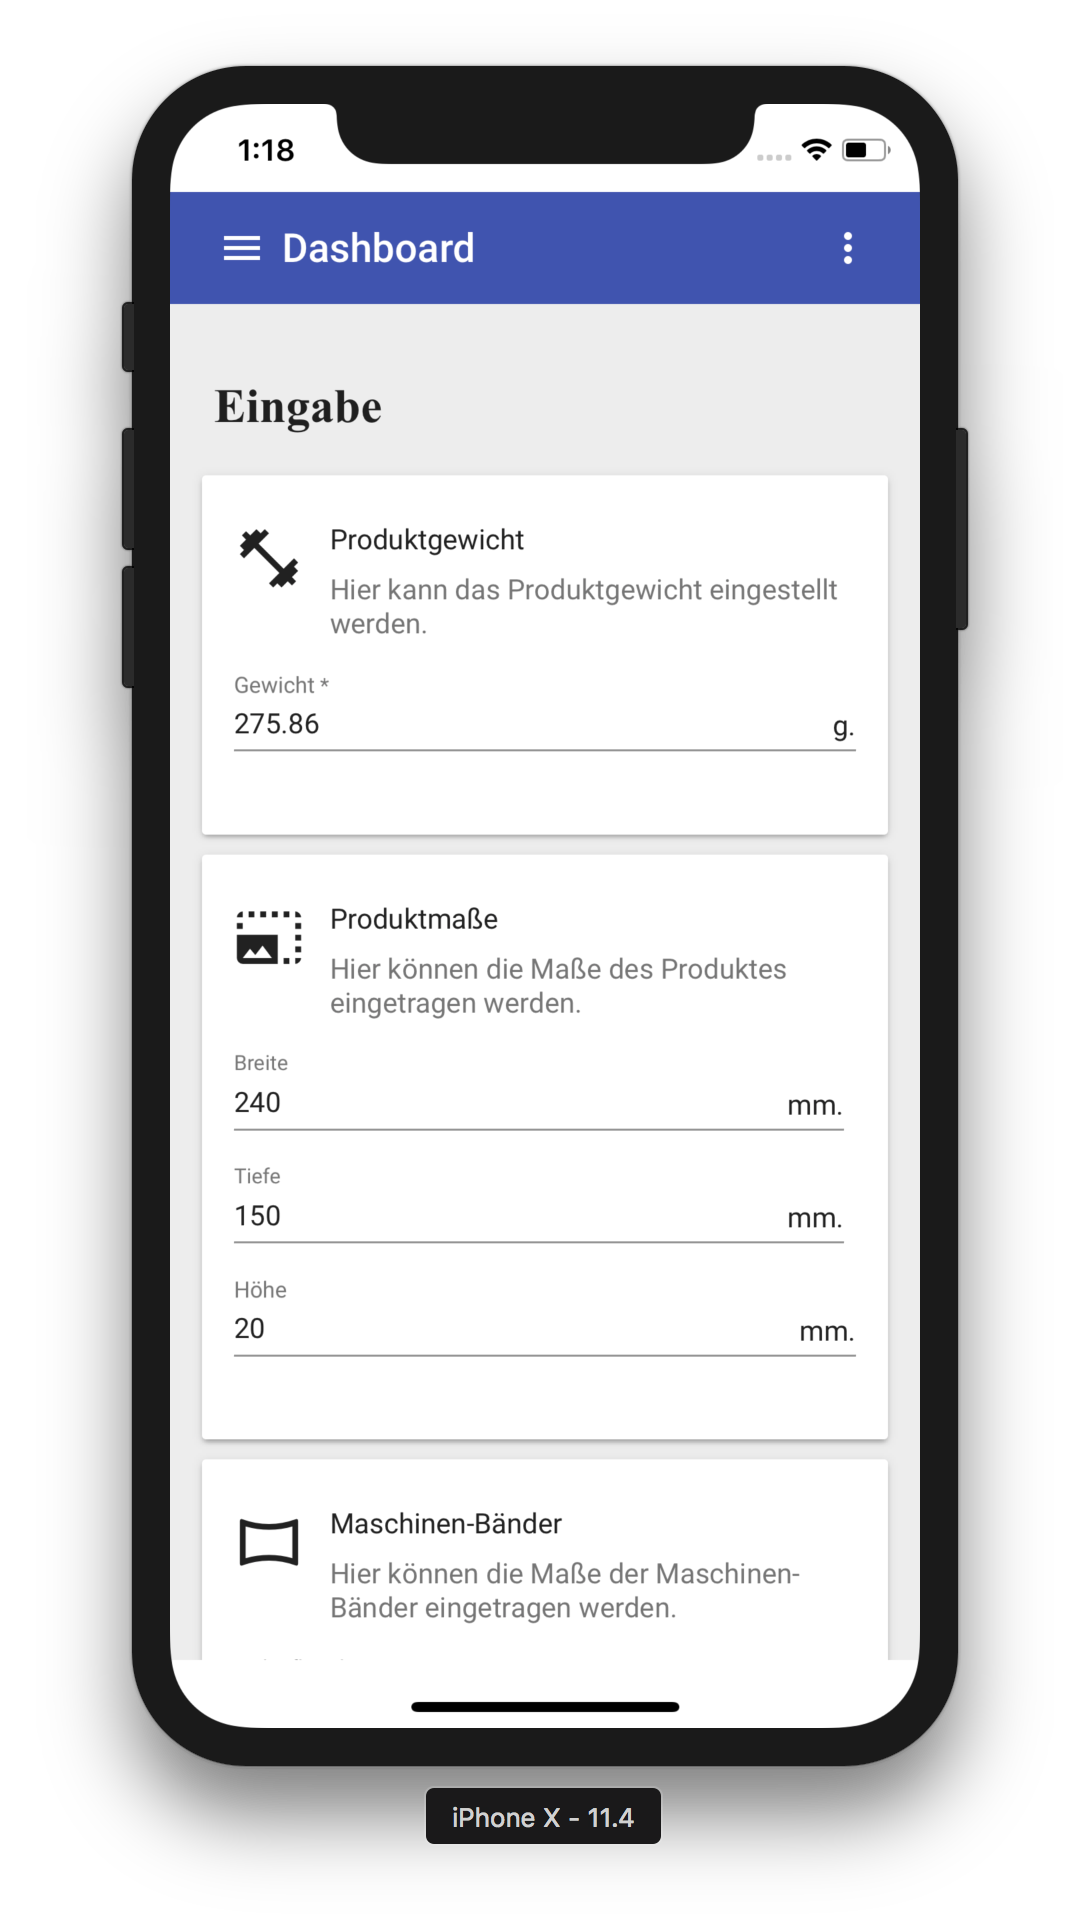
\includegraphics[scale=0.35]{images/kapitel_4/ios_app.png}
    \caption{iOS-App im Smartphone-Emulator}
    \label{fig:umsetzung_ios_app}
\end{figure}